\documentclass[12pt, TexShade, letterpaper]{report}

\usepackage[utf8]{inputenc}
\usepackage{palatino}
\usepackage{amsmath}
\usepackage{bm}
\usepackage{amssymb}
\usepackage{graphicx}
\usepackage[labelfont=bf]{caption}
\usepackage{subcaption}
\usepackage{setspace}
\captionsetup[table]{font = {stretch=1.35}}
\captionsetup[figure]{font = {stretch=1.35}}
\usepackage[margin=1in, headsep=1cm, bottom=5cm]{geometry}
\usepackage[hidelinks]{hyperref}
\newcommand{\MYhref}[3][blue]{\href{#2}{\color{#1}{#3}}}%
\usepackage{tabu}
\usepackage[table]{xcolor}
\usepackage{nomencl}
\usepackage{wrapfig}
\renewcommand{\baselinestretch}{2}
\usepackage{fancyhdr}
\usepackage{lmodern}
\usepackage{minted}
\usepackage{booktabs}
\usepackage[section]{placeins}
\usepackage{float}
\usepackage[style=ieee]{biblatex}
\usepackage{url}
\usepackage{amsthm}
\usepackage{array}

\addbibresource{references.bib}

\renewcommand{\chaptermark}[1]{\markboth{#1}{}} % Ensure List of Figs, ToC, and glossary are named in the header

% Overwrite the plain page style with a red line and page numbering
\fancypagestyle{plain}{%
	\fancyhf{} % clear all header and footer fields
	\fancyhead[R]{\textbf{\thepage}} % except the center
}

% Create the fancy page style header
\pagestyle{fancy}
\fancyhf{}
\lhead{\textbf{\nouppercase{\leftmark}}}
\chead{}
\rhead{\textbf{\thepage}}


\usepackage{xpatch}
\xpretocmd\headrule{\color{red}}{}{\PatchFailed}

% Get rid of all dashed words
\tolerance=1
\emergencystretch=\maxdimen
\hyphenpenalty=10000
\hbadness=10000

% Set page numbering to roman
\setcounter{page}{2}\renewcommand{\thepage}{\roman{page}}
\setcounter{tocdepth}{1}

\author{\textcopyright Author, August, 2020}
\date{}

\begin{document}

\begin{titlepage}
		\begin{center}
			\vspace*{0.5cm}

			\LARGE
			\textbf{Modelling Baseball Exit Velocities with the Block Maxima Method}
			
			\vspace{1cm}
			
			\textit{Jules Lanari-Collard}
			
			\vspace{1.2cm}
			
			
\includegraphics[width=0.25\textwidth]{mcglogo.png}
			
			\Large
			MATH 598 Final Project
			
			\vspace{-5mm}
			McGill University
			
			\vspace{-5mm}
			Montr\'eal, Qu\'ebec, Canada
			
			\vspace{5mm}
			December 20, 2024
			\small
			\vspace{0.5cm}
			{\color{red} \hrule height 0.75mm}
			\vspace{0.2cm}
		\end{center}
\end{titlepage}

\setlength{\voffset}{2cm}
\renewcommand{\chaptermark}[1]{%
	\markboth{\thechapter.\ #1}{}}

 % Start of ToC, LoT, gls
	\tableofcontents\thispagestyle{plain}
    \clearpage
    \pagenumbering{arabic} % restart page numbers at one, now in arabic style

\chapter{Introduction}
\section{Process over Outcomes}
Baseball is the second-most popular sport in the United States \cite{gallupPoll}, and the average Major League Baseball (MLB) franchise is worth \$2.4 billion. Teams invest significant amounts on player wages every year, with the median projected payroll for 2025 being \$144 million, and some teams projected for over \$270 million \cite{fgRosterResource}. Salaries are often disproportionately concentrated in a small number of high-value players; Shohei Ohtani signed the largest contract in sports history, \$700 million over 10 years, in 2024 \cite{ohtaniContract}, and Juan Soto recently broke that record with a \$765 million, 15 year contract with the New York Mets \cite{sotoContract}.

With the amounts of money involved, franchises employ dedicated analytics teams within their front offices to inform decisions and evaluate and project players. Having a good understanding of a player's current and future ability is not only important when signing them to a large free agent contract, but also when trying to identify undervalued players.

Since the introduction of Statcast technology to MLB in 2015, allowing high-resolution ball and player tracking every game, there has been a shift in perspective on player evaluation. The technology allows analysts to evaluate events with respect to the \textit{process}, not just the results. Instead of considering a ball in play as a binary event, either resulting in a hit or an out, we can consider the \textit{expected outcome} in a probabilistic sense, given various factors such as the launch speed and launch angle. Over the course of many seasons, the wealth of data generated with this perspective has enabled a better separation between a player's true talent and luck and random variance; parsing the signal from the noise.

\section{The Importance of Exit Velocity}
One such Statcast metric is launch speed (more commonly known as \textbf{exit velocity}), simply measuring the speed (in mph) at which the baseball travels immediately after being hit by the bat. On a player level this has helped to quantify player `power'. The use of this metric is rather intuitive; harder hit balls are more likely to turn into hits and even home runs. Figure \ref{fig:woba-ev} demonstrates this effect, using \textbf{wOBACON}\footnote{wOBACON stands for \textit{Weighted On-Base Average on CONtact}. We will not go into the details of its calculation, but the main takeaway is that it measures the value of the outcomes of balls in play. For example, hits and home runs are positive, whilst outs are 0.} as a measure for outcome value, demonstrating an interesting trend; balls in play under 75mph all perform similarly, but above 75mph there is a clear positive correlation between exit velocity (EV) and quality of outcome.

\begin{figure}[h]
    \centering
    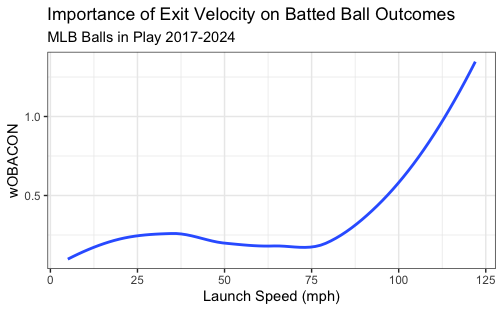
\includegraphics[width=0.75\linewidth]{plots/ev_woba.png}
    \caption{wOBACON and Exit Velocity}
    \label{fig:woba-ev}
\end{figure}

From the perspective of player evaluation, it follows that we can expect hitters who are able to consistently hit the ball harder to perform better. The question then turns to how can we best interpret each player's exit velocity data on a larger scale. To give an extreme example, suppose player A hits every ball at 100mph, whilst player B hits 80\% of their batted balls at 95mph and the remaining 20\% at 120mph. It is unclear which player provides more value; they have equal \textit{average} exit velocities, but the value of their outcomes is not necessarily the same. Indeed, players across the league exhibit very different exit velocity distributions, and designing metrics to describe these distributions is a topic of great debate. Figure \ref{fig:player-comp} illustrates the difference in distribution shape between two highly contrasting players.

\begin{figure}
    \centering
    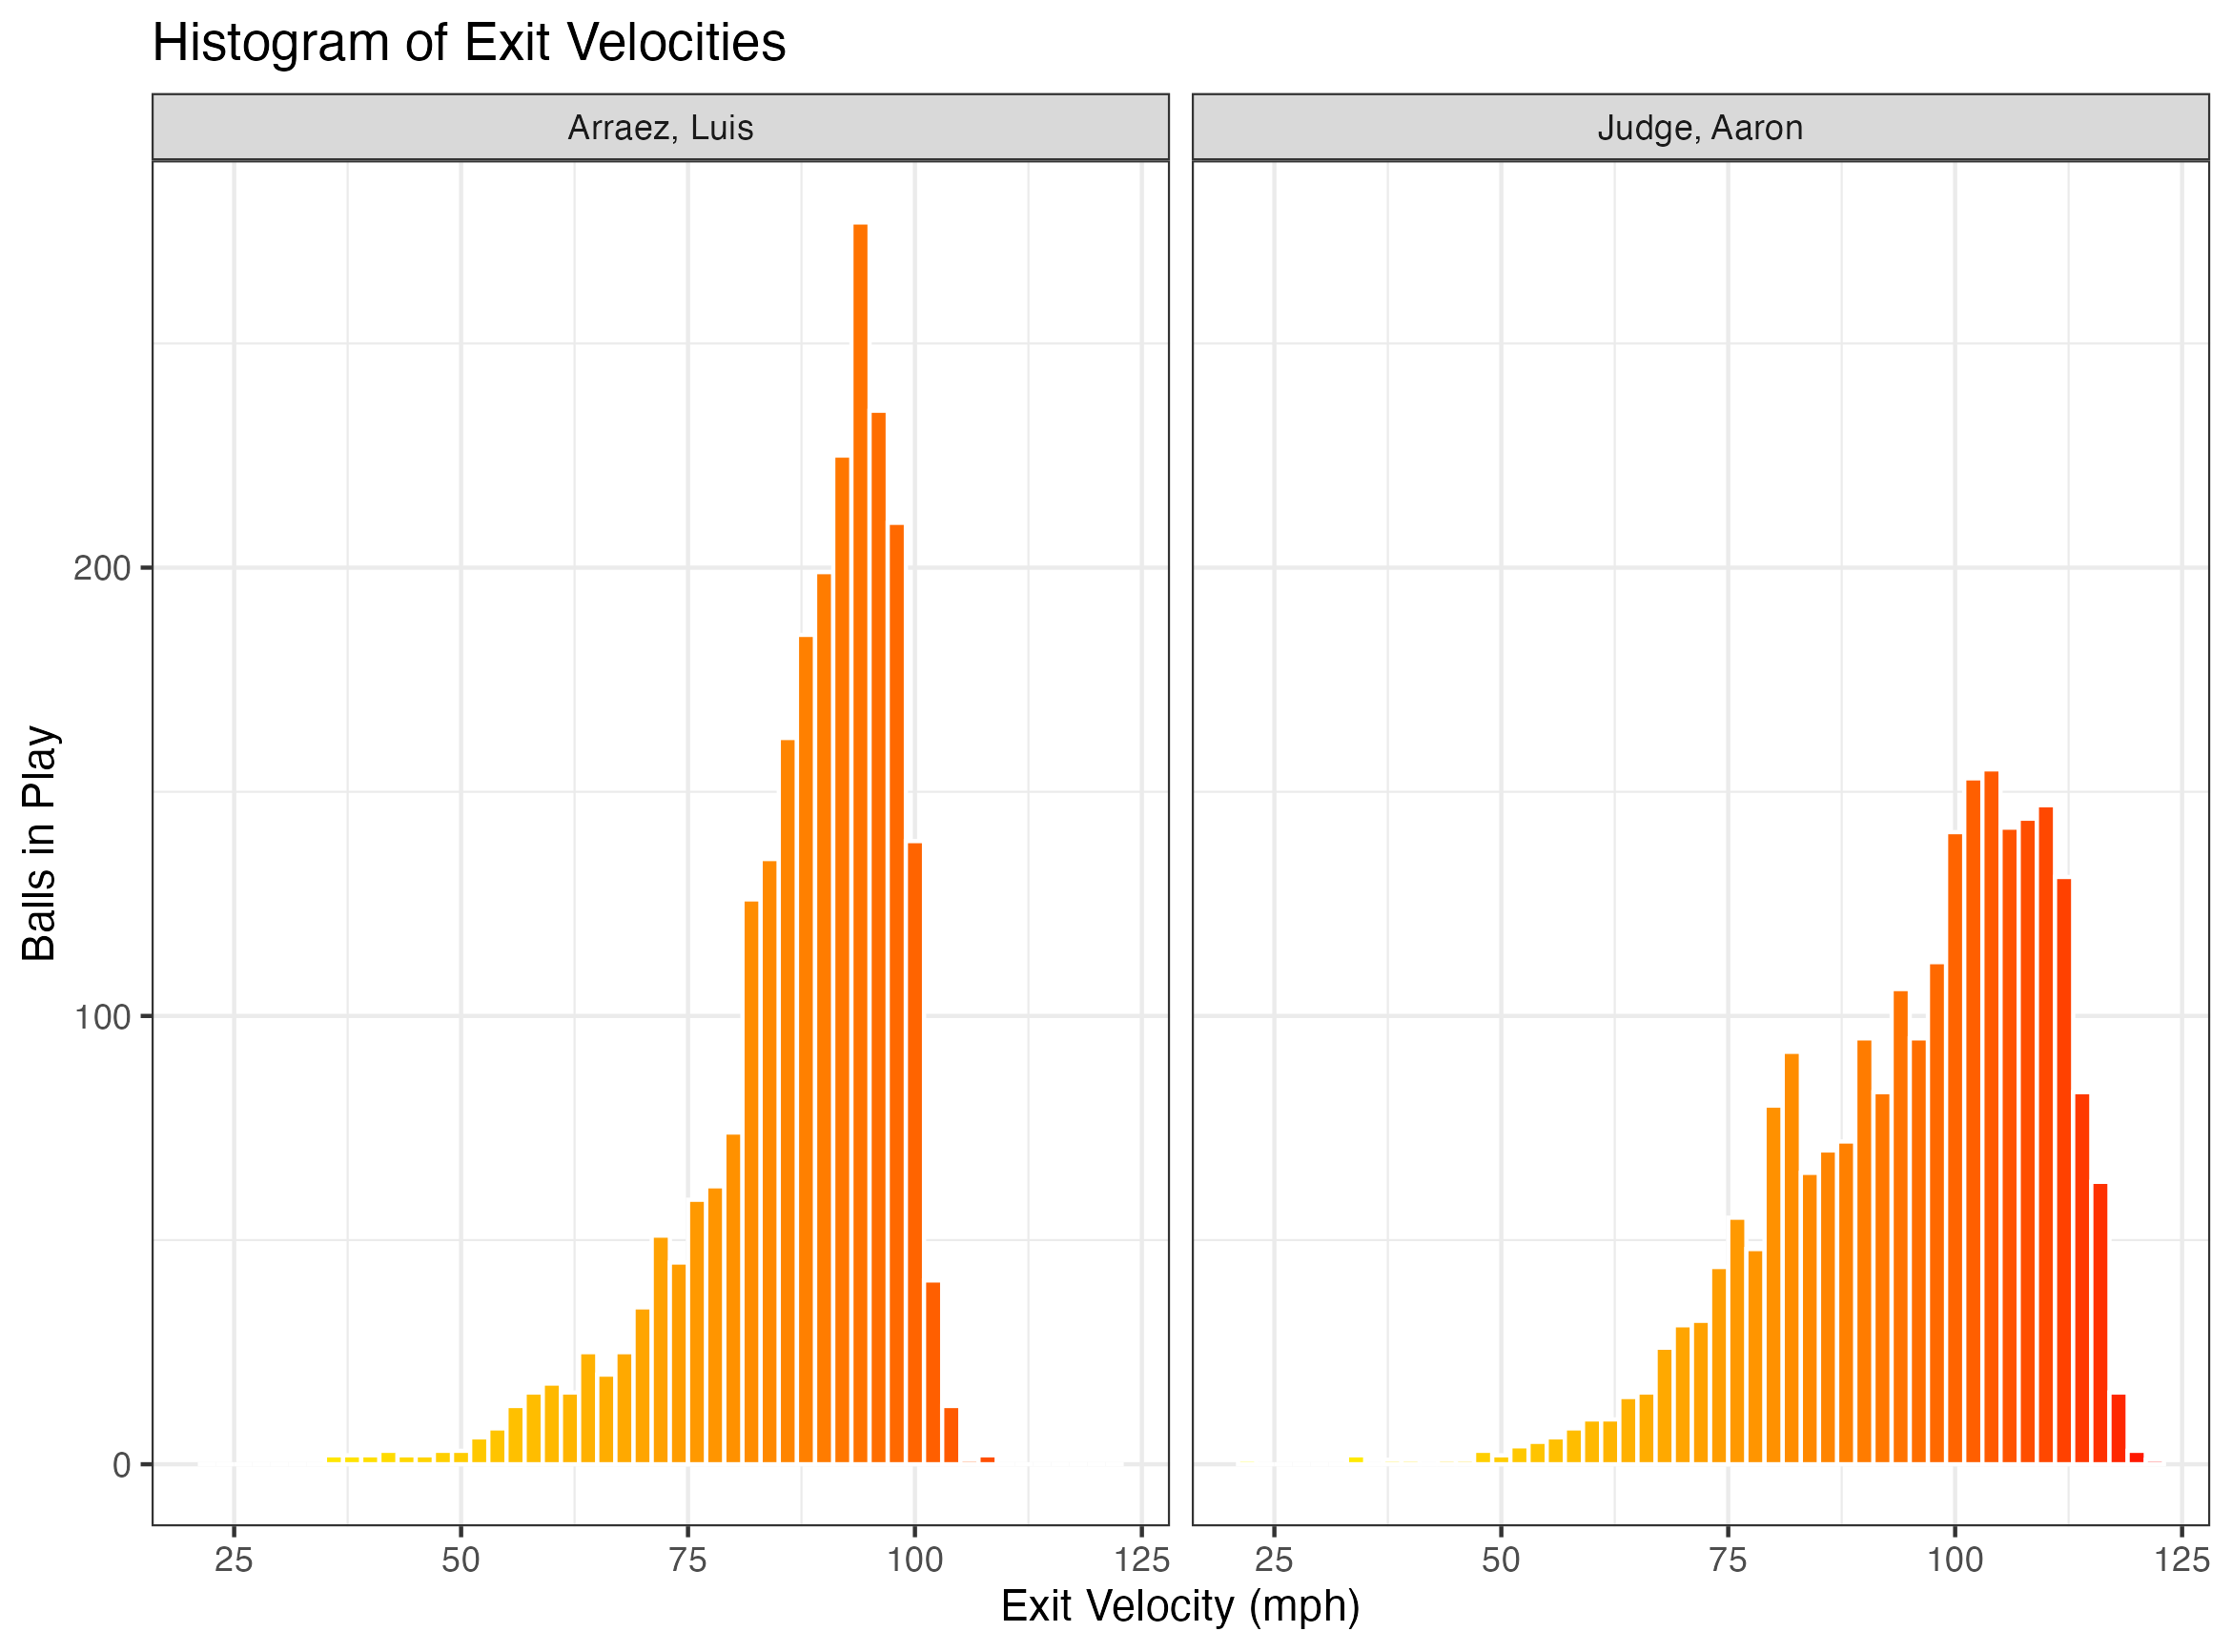
\includegraphics[width=0.8\linewidth]{plots/playerComparison.png}
    \caption{Comparison of Contrasting EV Distributions}
    \label{fig:player-comp}
\end{figure}

\section{Summarising Exit Velocity Data}\label{metrics}
Attempting to effectively summarise player-level exit velocity data, many metrics have already been formulated, with differing degrees of complexity. Before discussing the existing metrics, it is important to discuss what qualifies as an `informative' or `useful' metric. Metrics can be generally evaluated on three main criteria:
\begin{itemize}
    \item Correlation with outcomes: how well does a metric represent value?
    \item Correlation with future outcomes: how well does a metric predict future outcomes and value?
    \item Variance: how much does a metric vary from year-to-year? In other words, how susceptible is the metric to random noise? In the search to separate true talent from randomness, low-variance (so-called `sticky') metrics are much more reliable due to their robustness against random variation of the underlying data.
\end{itemize}

\subsection{Existing Metrics}
\subsubsection{Average Exit Velocity}
Self-explanatory in its definition, average EV is generally viewed as a flawed statistic, as it is equally affected by both the lower and upper quantiles of a player's EV distribution. As seen in Figure \ref{fig:woba-ev}, balls hit slower than 75mph should be viewed as roughly equal in value, and do not provide as much information as the upper quantiles.

\subsubsection{Best Speed}
In response to the flaws of average EV, Tom Tango stated that we ``learn nothing about a batter on their slow hit batted balls" \cite{tangoBestSpeed}, and instead proposed \textbf{best speed}, defined as the average of a batter's top 50\% hardest-hit balls. Best speed correlates better with outcomes and exhibits less year-to-year variation than average EV \cite{andrewsEV}.

\subsubsection{Exit Velocity Percentiles}
Alternatively, one can consider the empirical quantiles of a player's exit velocities. Commonly used quantiles are the 80th, 90th and 95th percentiles, known as \textbf{EV80}, \textbf{EV90} and \textbf{EV95} respectively \cite{clemensEV}. They perform similarly to best speed in correlation with outcomes and predictive power, and are even lower variance than best speed.

\subsubsection{Maximum Exit Velocity}
Also self-explanatory, maximum EV is simply the speed of a player's hardest-hit ball over a given period of time, typically a season. Unsurprisingly, due to its inefficient use of information, it performs worse than the aforementioned metrics in correlation with outcomes, predictive power, and is only lower in variance than average EV.

\section{Applying Extreme Value Theory}
In summary, exit velocity data has a number of traits which render it difficult to analyse with traditional methods:
\begin{itemize}
    \item EV distributions vary drastically from player to player, not only in parameters but also potentially in type of distribution.
    \item We learn very little about a player's true talent from their slowly-hit batted balls (i.e. bottom 50\%).
    \item Information about player talent lies in upper quantiles of their EV distribution.
\end{itemize}
Given that individual batted ball events (and thus also their block maxima) can safely be assumed to be i.i.d.\footnote{This was verified using an auto-correlation plot.}, extreme value theory is particularly suited to this problem. Although player-level EV distributions may differ greatly, their block-maxima will follow a Generalised Extreme Value (GEV) distribution, allowing us to fit a model for each player without restrictive assumptions on their underlying EV distribution.

\chapter{Methods}
\section{Data}
Data was collected using queries to the MLB Statcast Search API\footnote{Accessible at \url{https://baseballsavant.mlb.com/statcast_search}}, querying all balls in play from 2015 (implementation of Statcast tracking) to 2024. The full dataset consists of 1,157,634 batted ball events involving 2,373 unique hitters. 2,020 player seasons consisted of at least 250 batted ball events (BBEs), a threshold set to ensure sufficient sample size for good model fits in the ensuing analysis.

\section{Block Maxima}
Seeking to model the upper quantiles of each player's exit velocity distribution, we use the block-maxima method to fit a GEV model to the data. An alternative approach would be the Peaks-Over-Threshold (POT) method, however threshold selection is a complex problem, and not generalisable when looking to fit a model for each player. With the block-maxima method, we can set a constant block size for all models without overly adverse effects on the model fit.

The GEV parameters can be estimated using maximum likelihood methods with the \mintinline{R}{ismev} package \cite{ismev} in \textit{R}. Using only player seasons with at least 250 BBEs, a model was fitted for each player season (2,020 total) using a block size of 10 balls in play. The distributions of the estimated parameters are shown in Figure \ref{fig:params}. The parameter of interest for evaluating the quality of the models is the shape (denoted $\xi$); MLE is not well-behaved for $\xi \in (-1, -\frac{1}{2}]$ and potentially unobtainable when $\xi \leq -1$. The software implementation did not encounter issues, although over 50\% of the estimates having $\hat{\xi} \leq -\frac{1}{2}$ is a cause for concern.

\begin{figure}[ht]
    \centering
    \begin{subfigure}[]{0.45\textwidth}
        \centering
        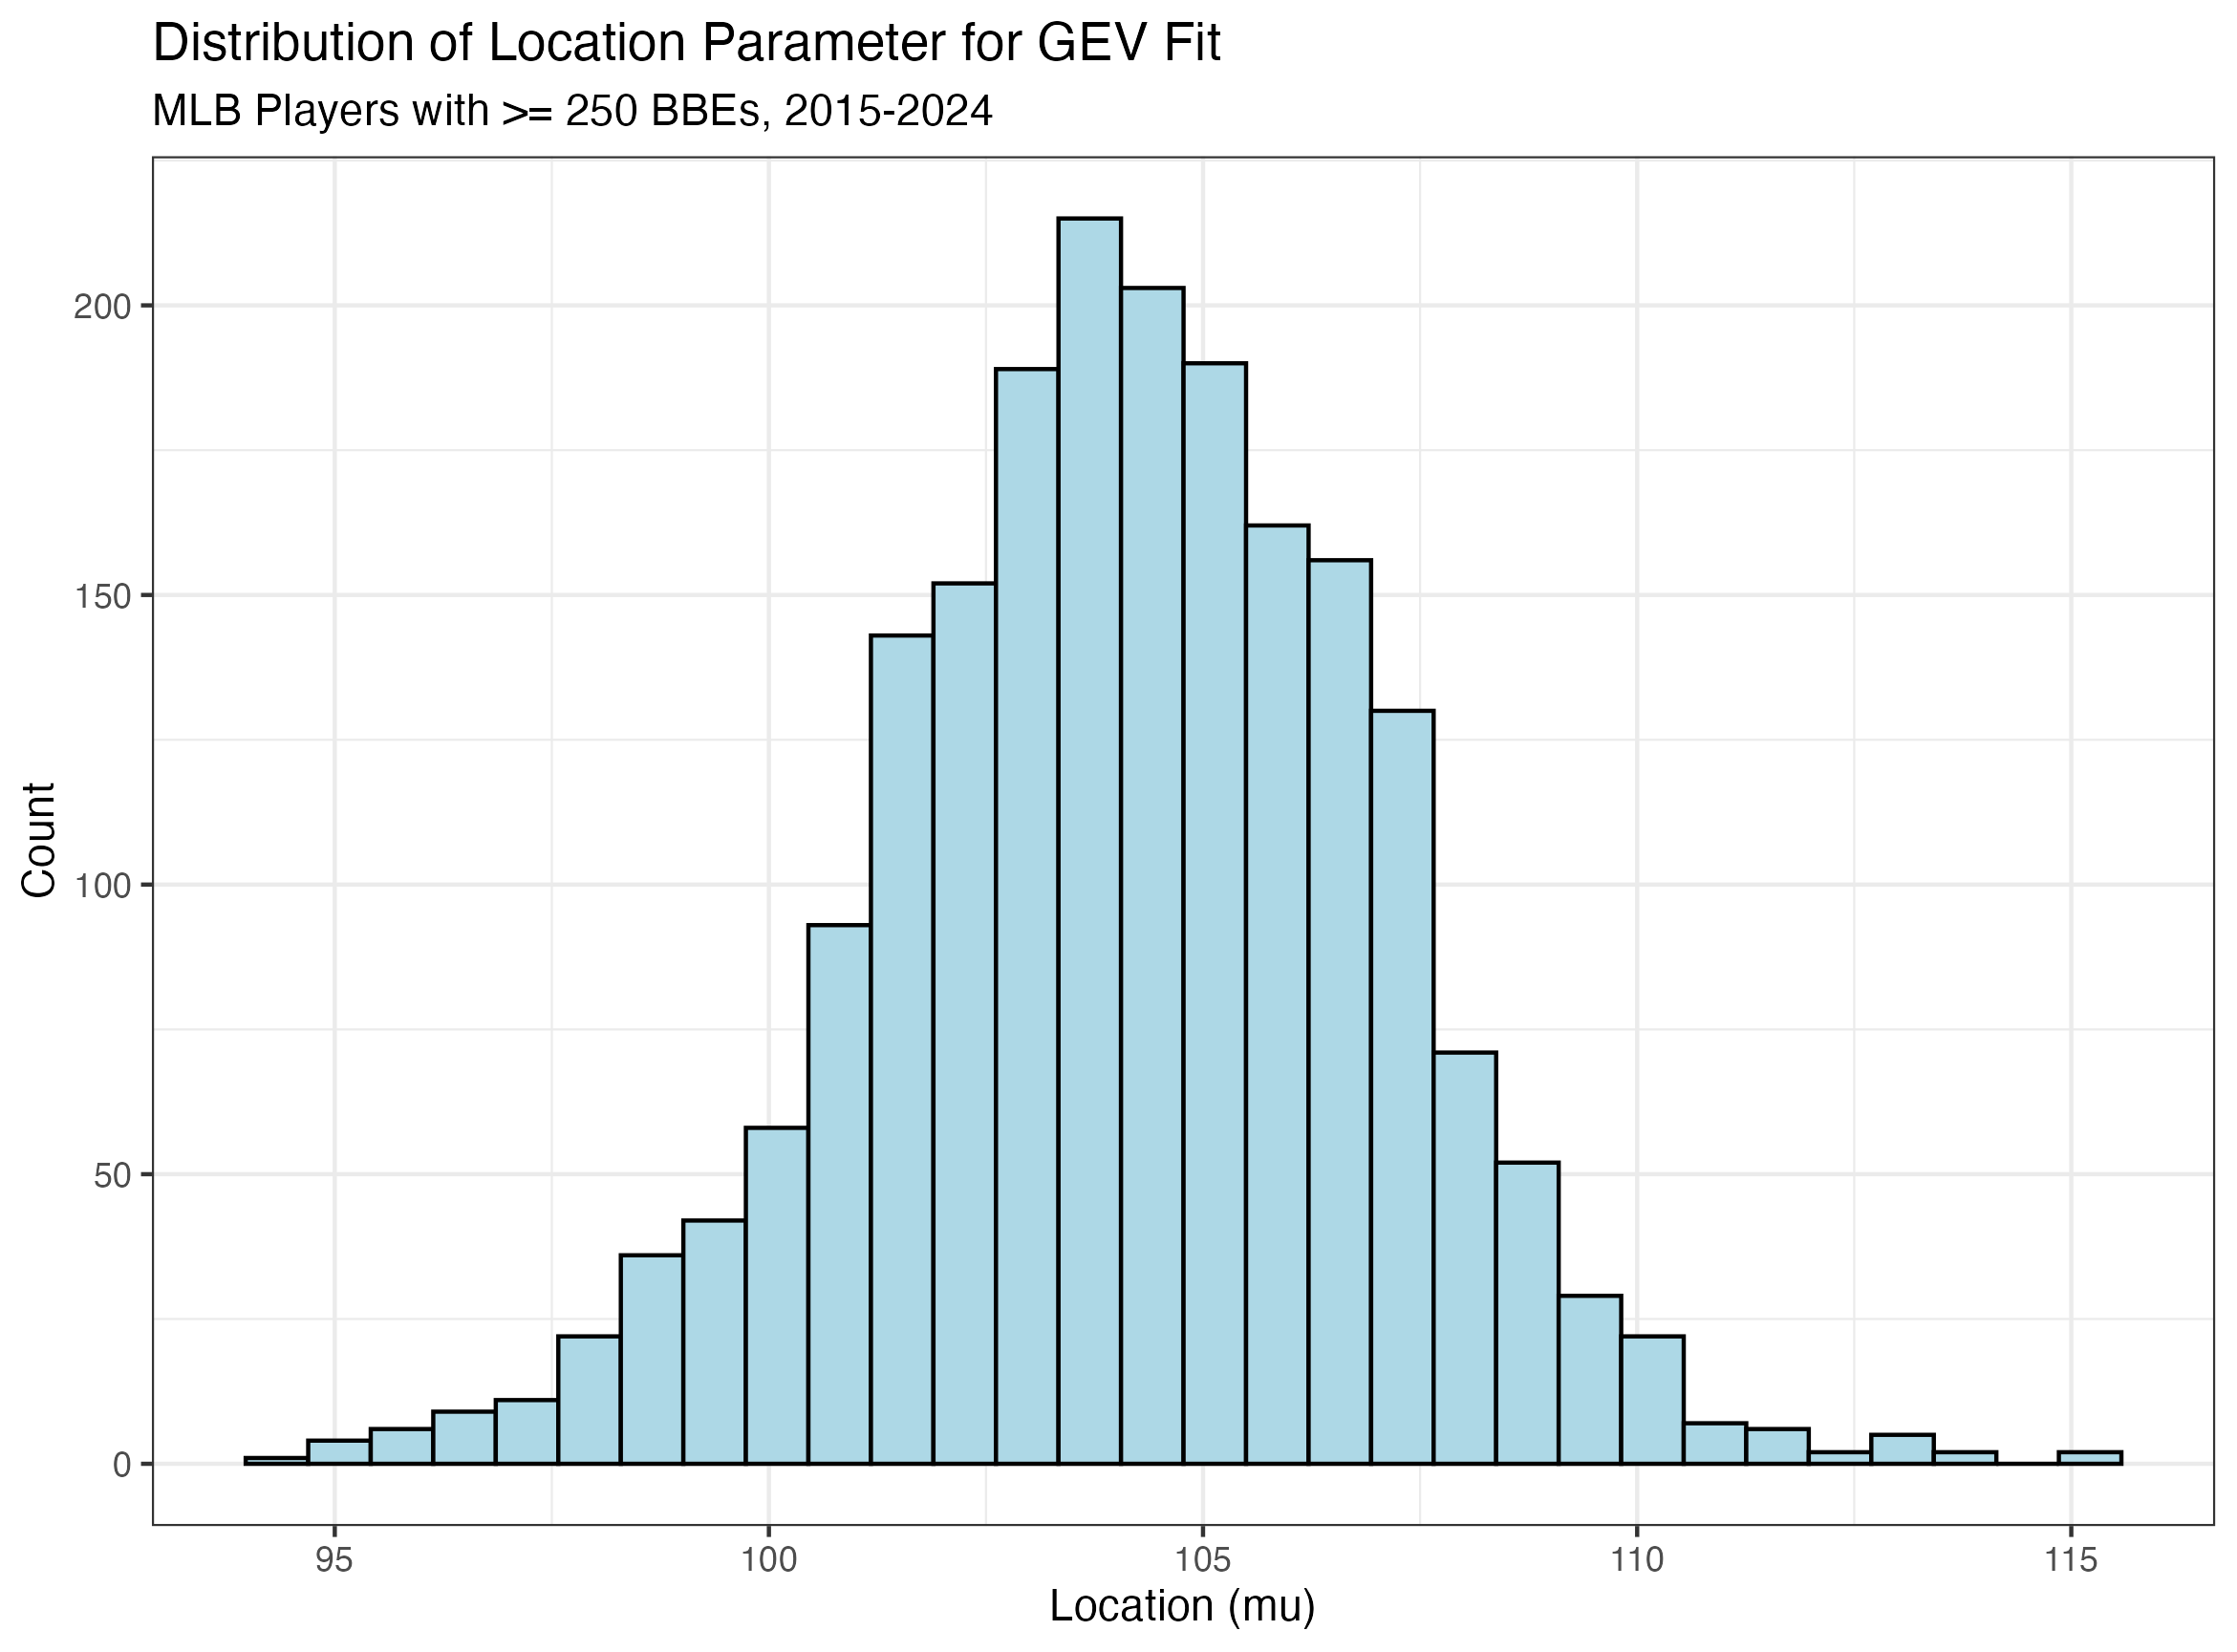
\includegraphics[width=\textwidth]{plots/location.png}
        \caption{Location}
    \end{subfigure}
    \begin{subfigure}[]{0.45\textwidth}
        \centering
        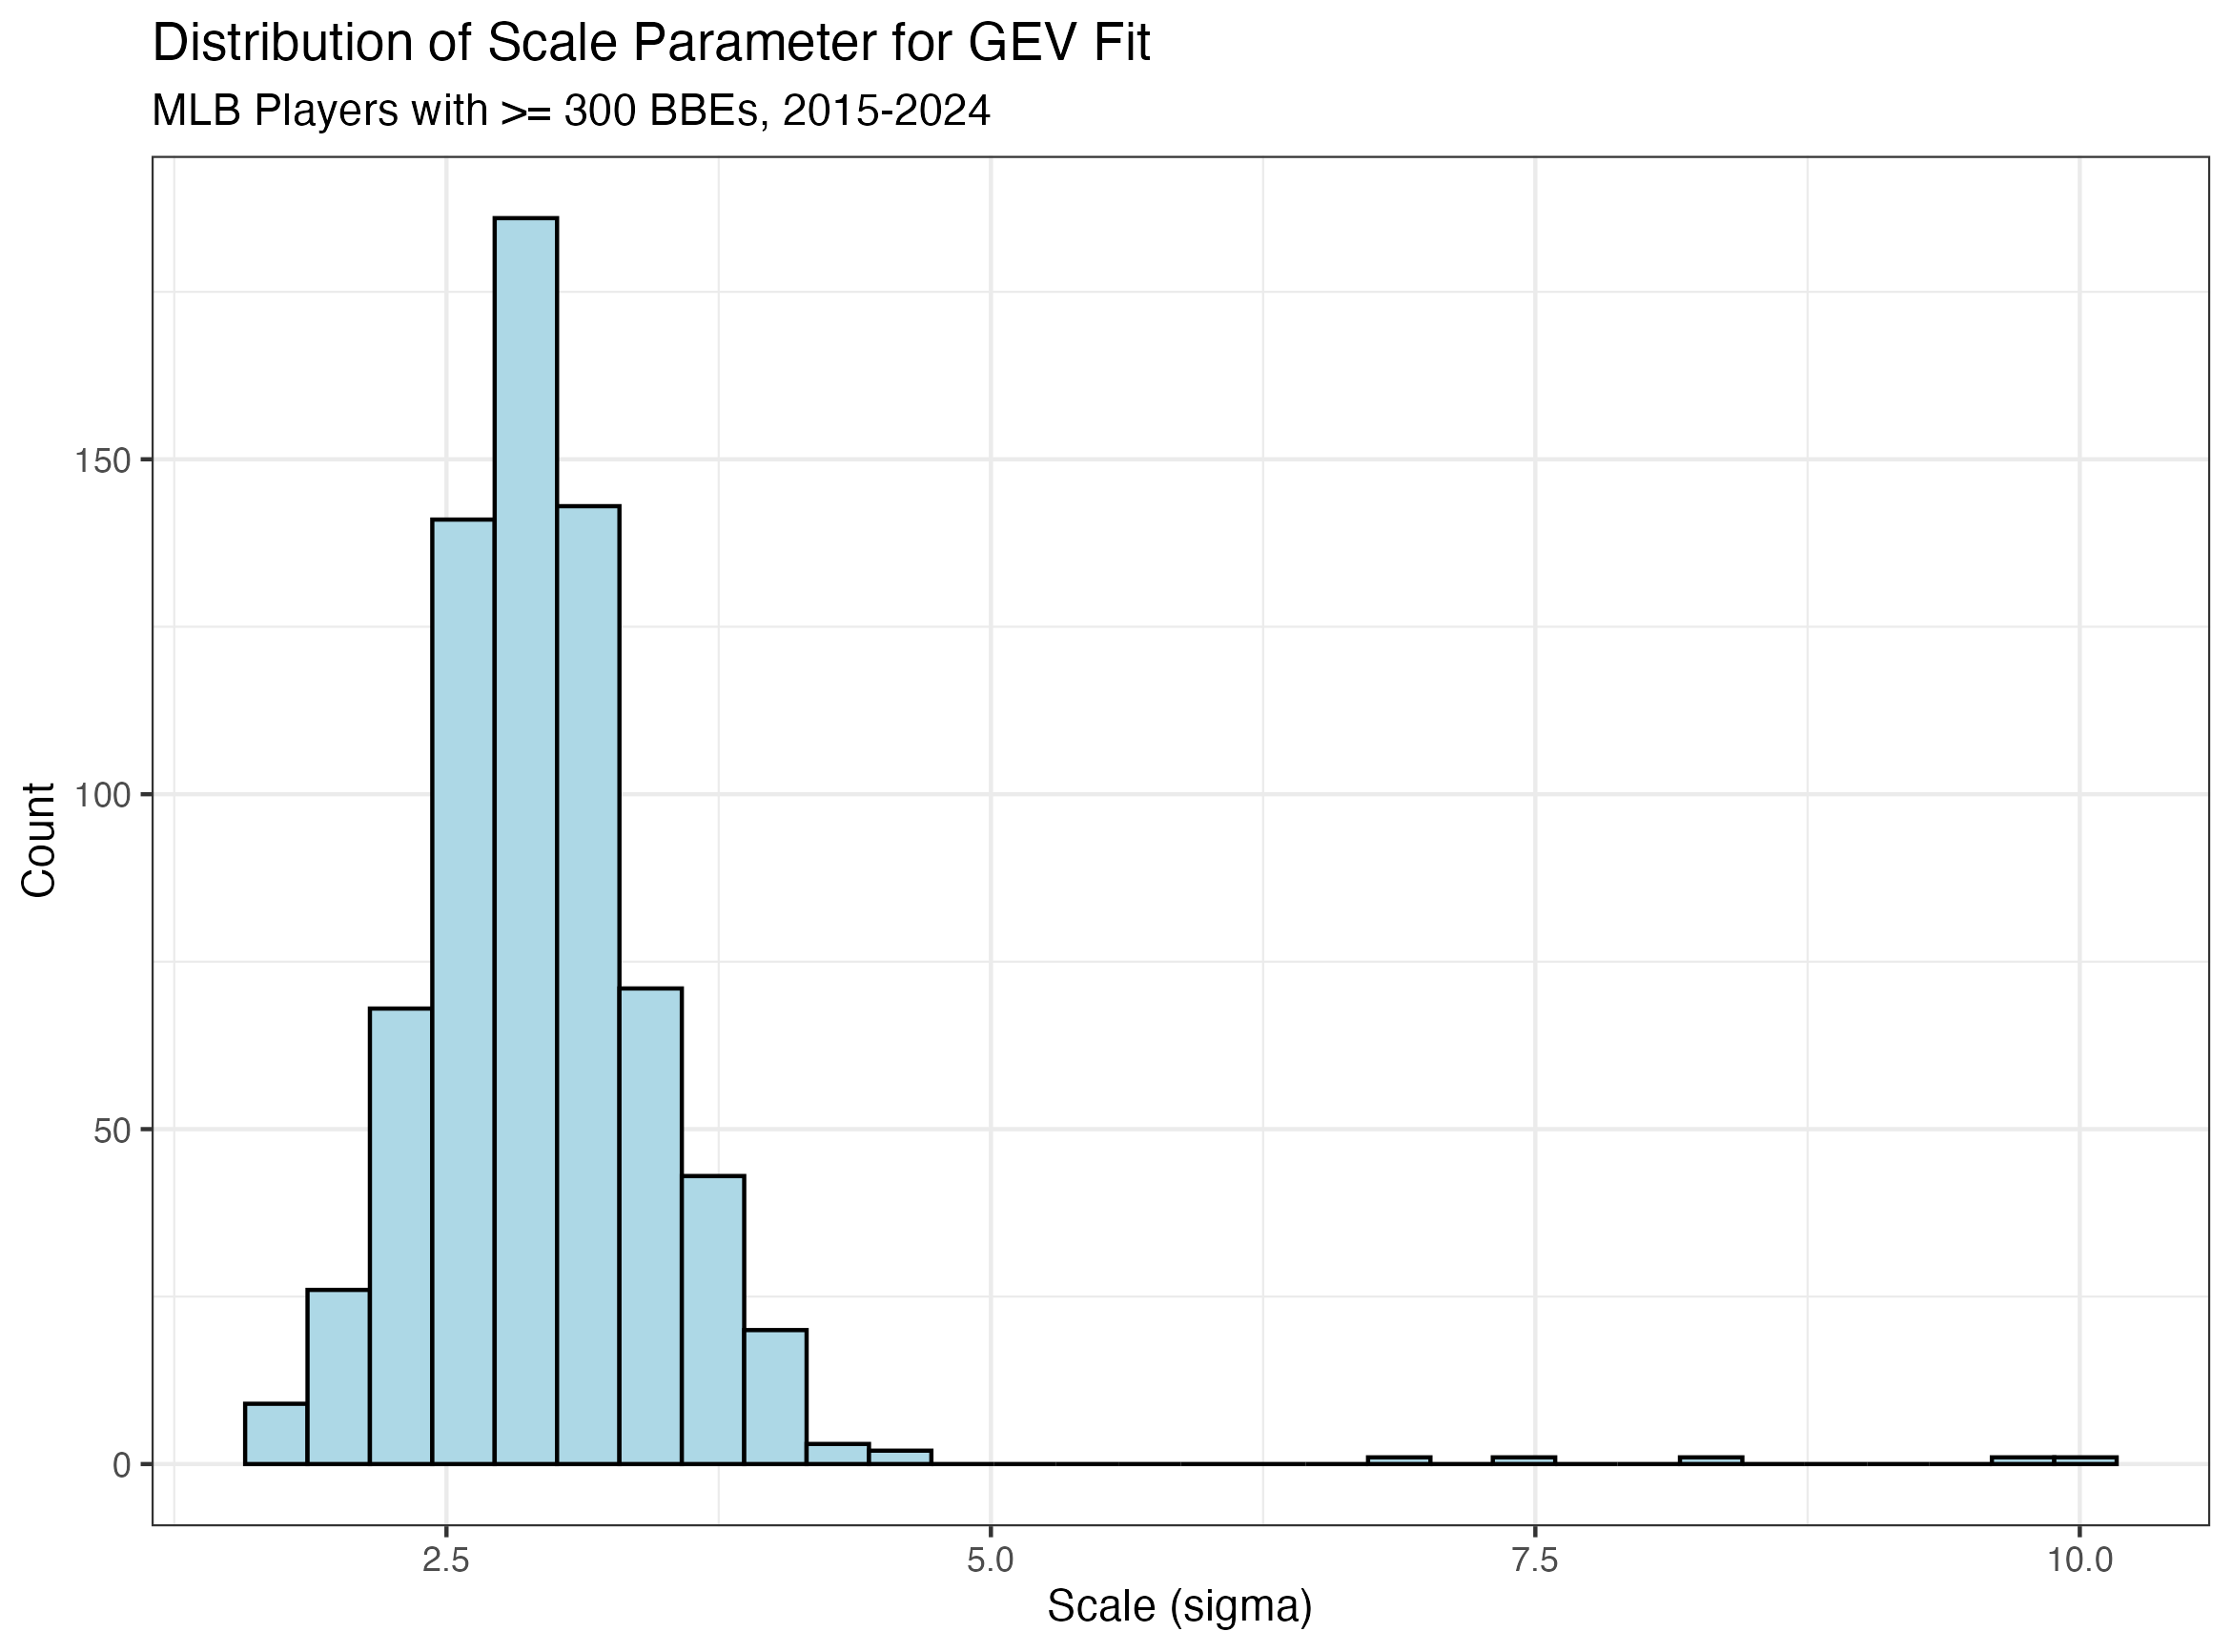
\includegraphics[width=\textwidth]{plots/scale.png}
        \caption{Scale}
    \end{subfigure}
    \begin{subfigure}[]{0.45\textwidth}
        \centering
        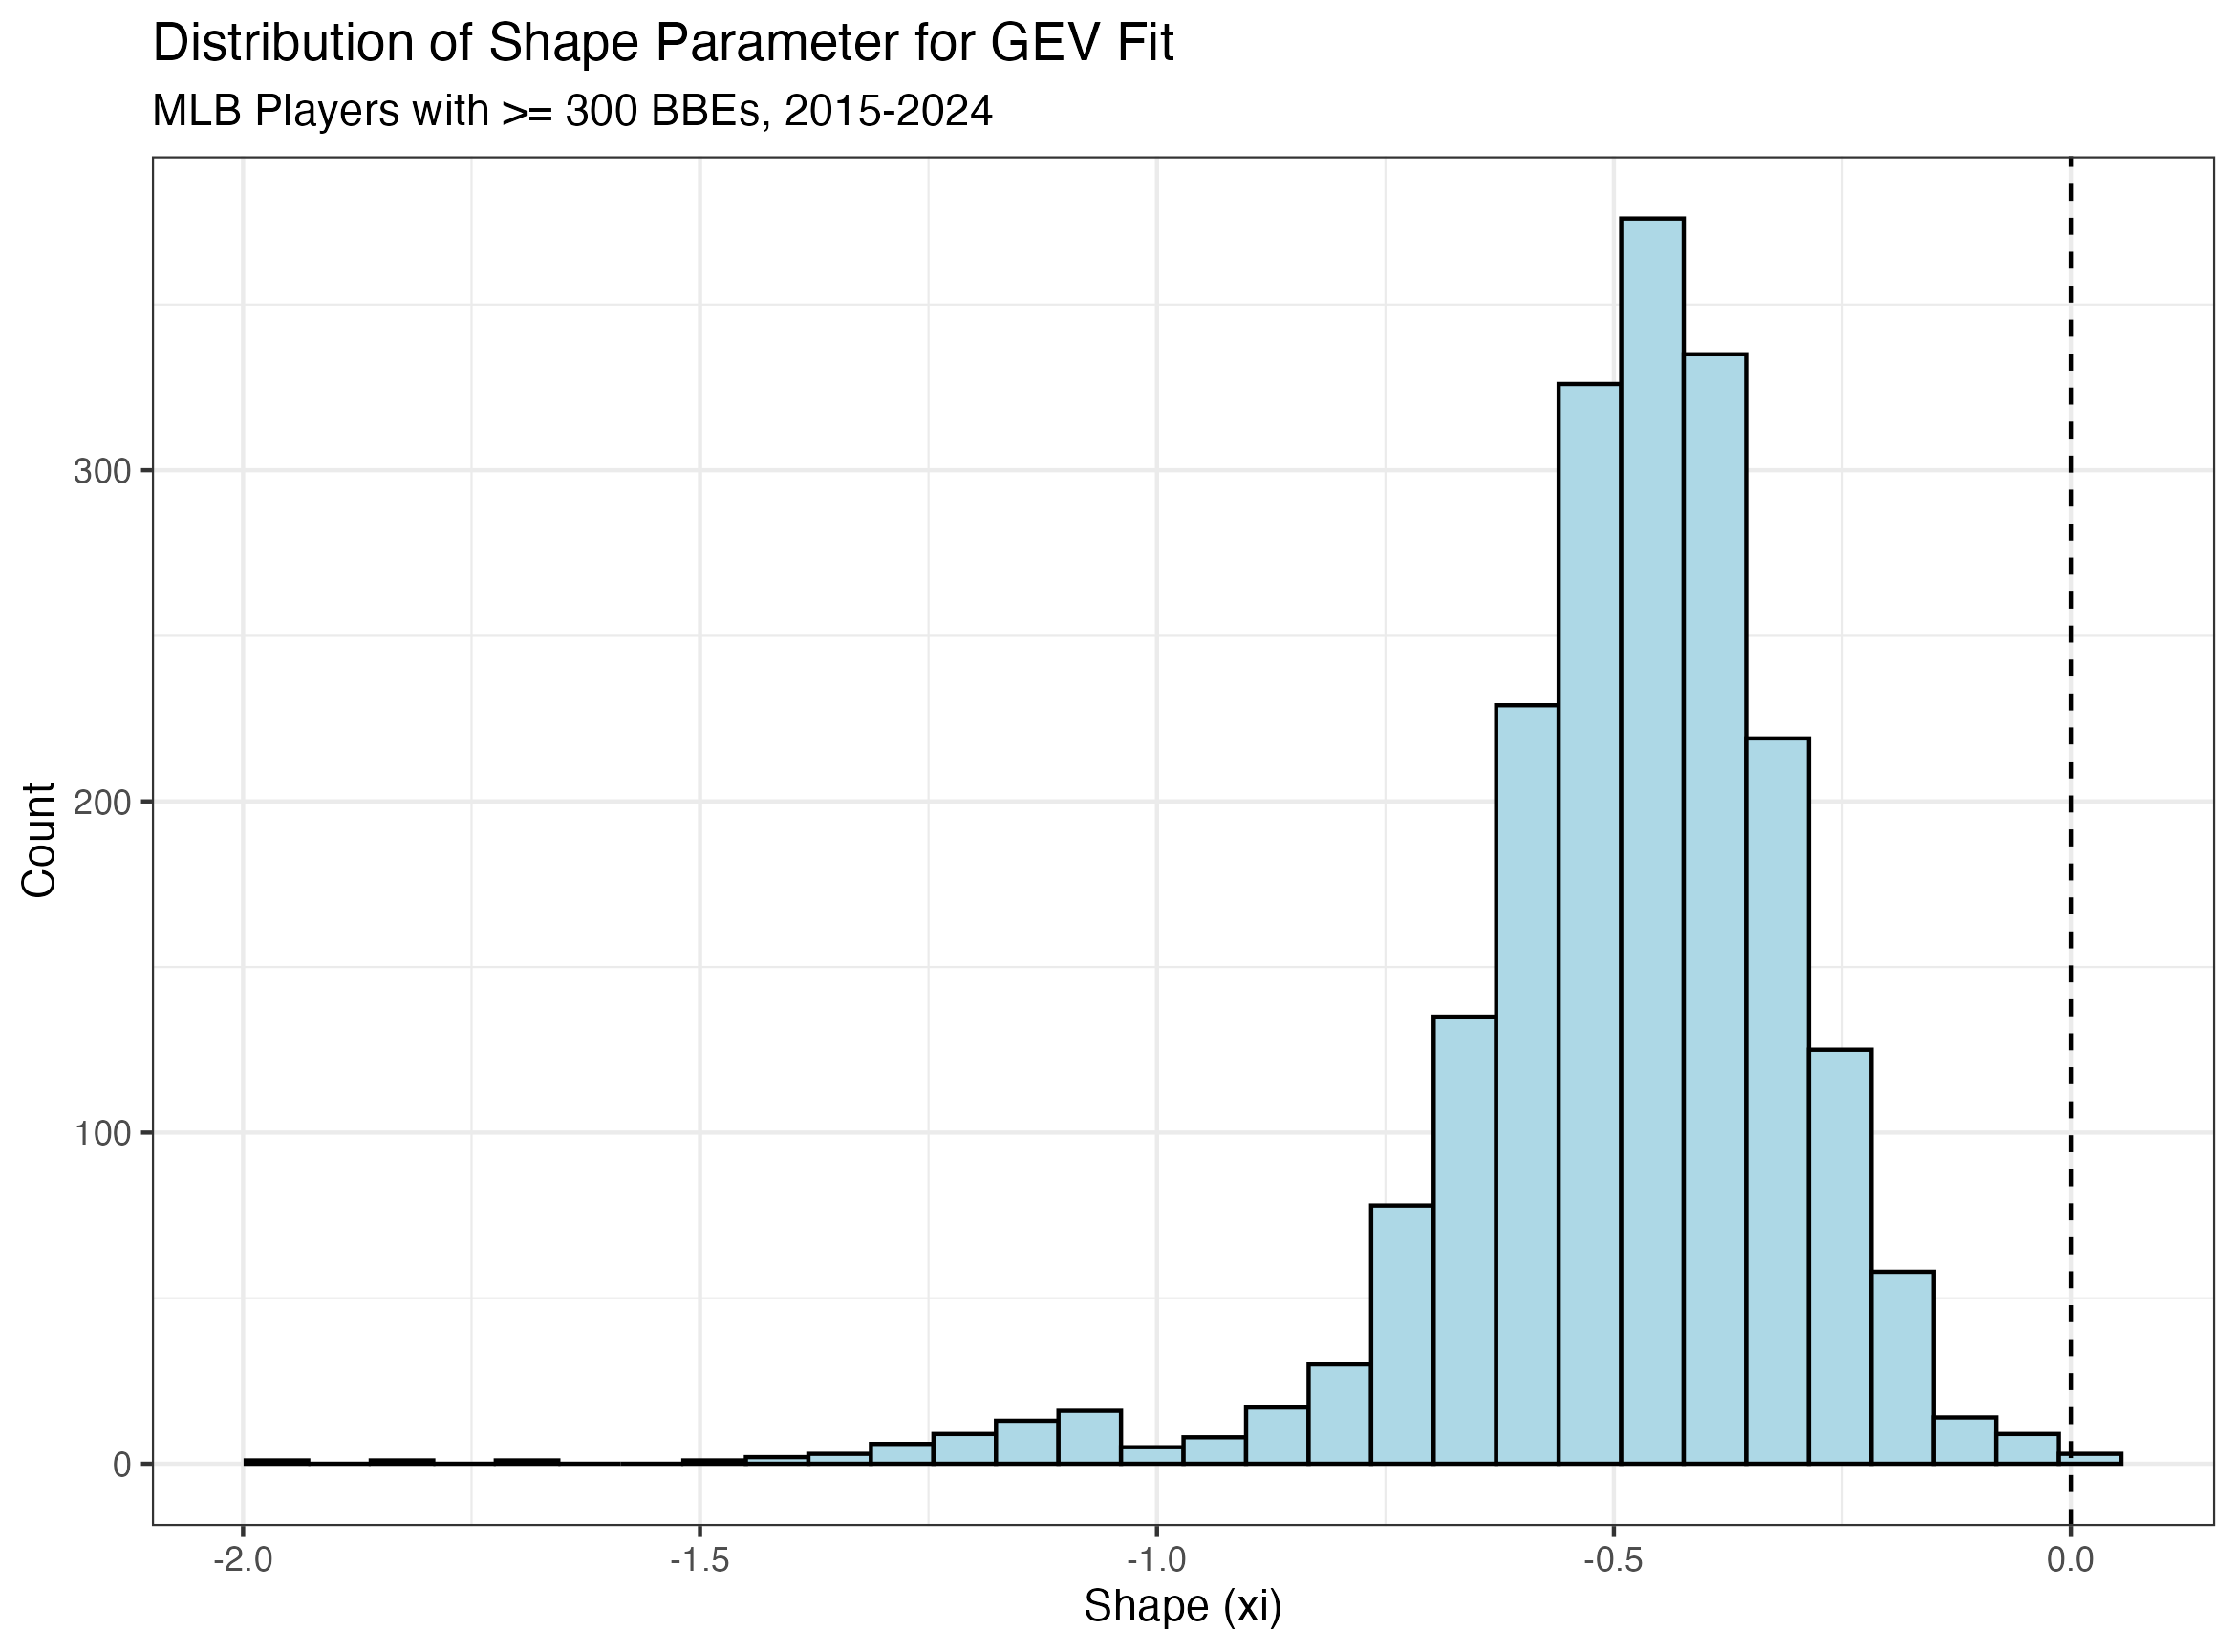
\includegraphics[width=\textwidth]{plots/shape.png}
        \caption{Shape}
    \end{subfigure}
    \caption{Distribution of Estimated Parameters}
    \label{fig:params}
\end{figure}

When evaluating the fit of an individual GEV model, one can use visual diagnostic tools such as q-q plots and probability plots, however this becomes unfeasible when evaluating such a large number of models. Alternatively, we can use the well-known fact that the transform of a random sample drawn from a CDF $F$ with $F$ itself is standard uniformly distributed\footnote{The inverse of this process is known as the inverse transform method, used for generating random samples from different distributions.}. With this in mind, for each player season, we transform the block maxima with the GEV CDF with the estimated parameters. For a well-fitted model, the resulting points should be approximately standard uniform, which we can test with the Kolmogorov-Smirnov Test for Uniformity. The p-values this test on each model are displayed in Figure \ref{fig:ks-test}, where we see that most of the transforms are in fact normally distributed at the 5\% significance level.

\begin{figure}[ht]
    \centering
    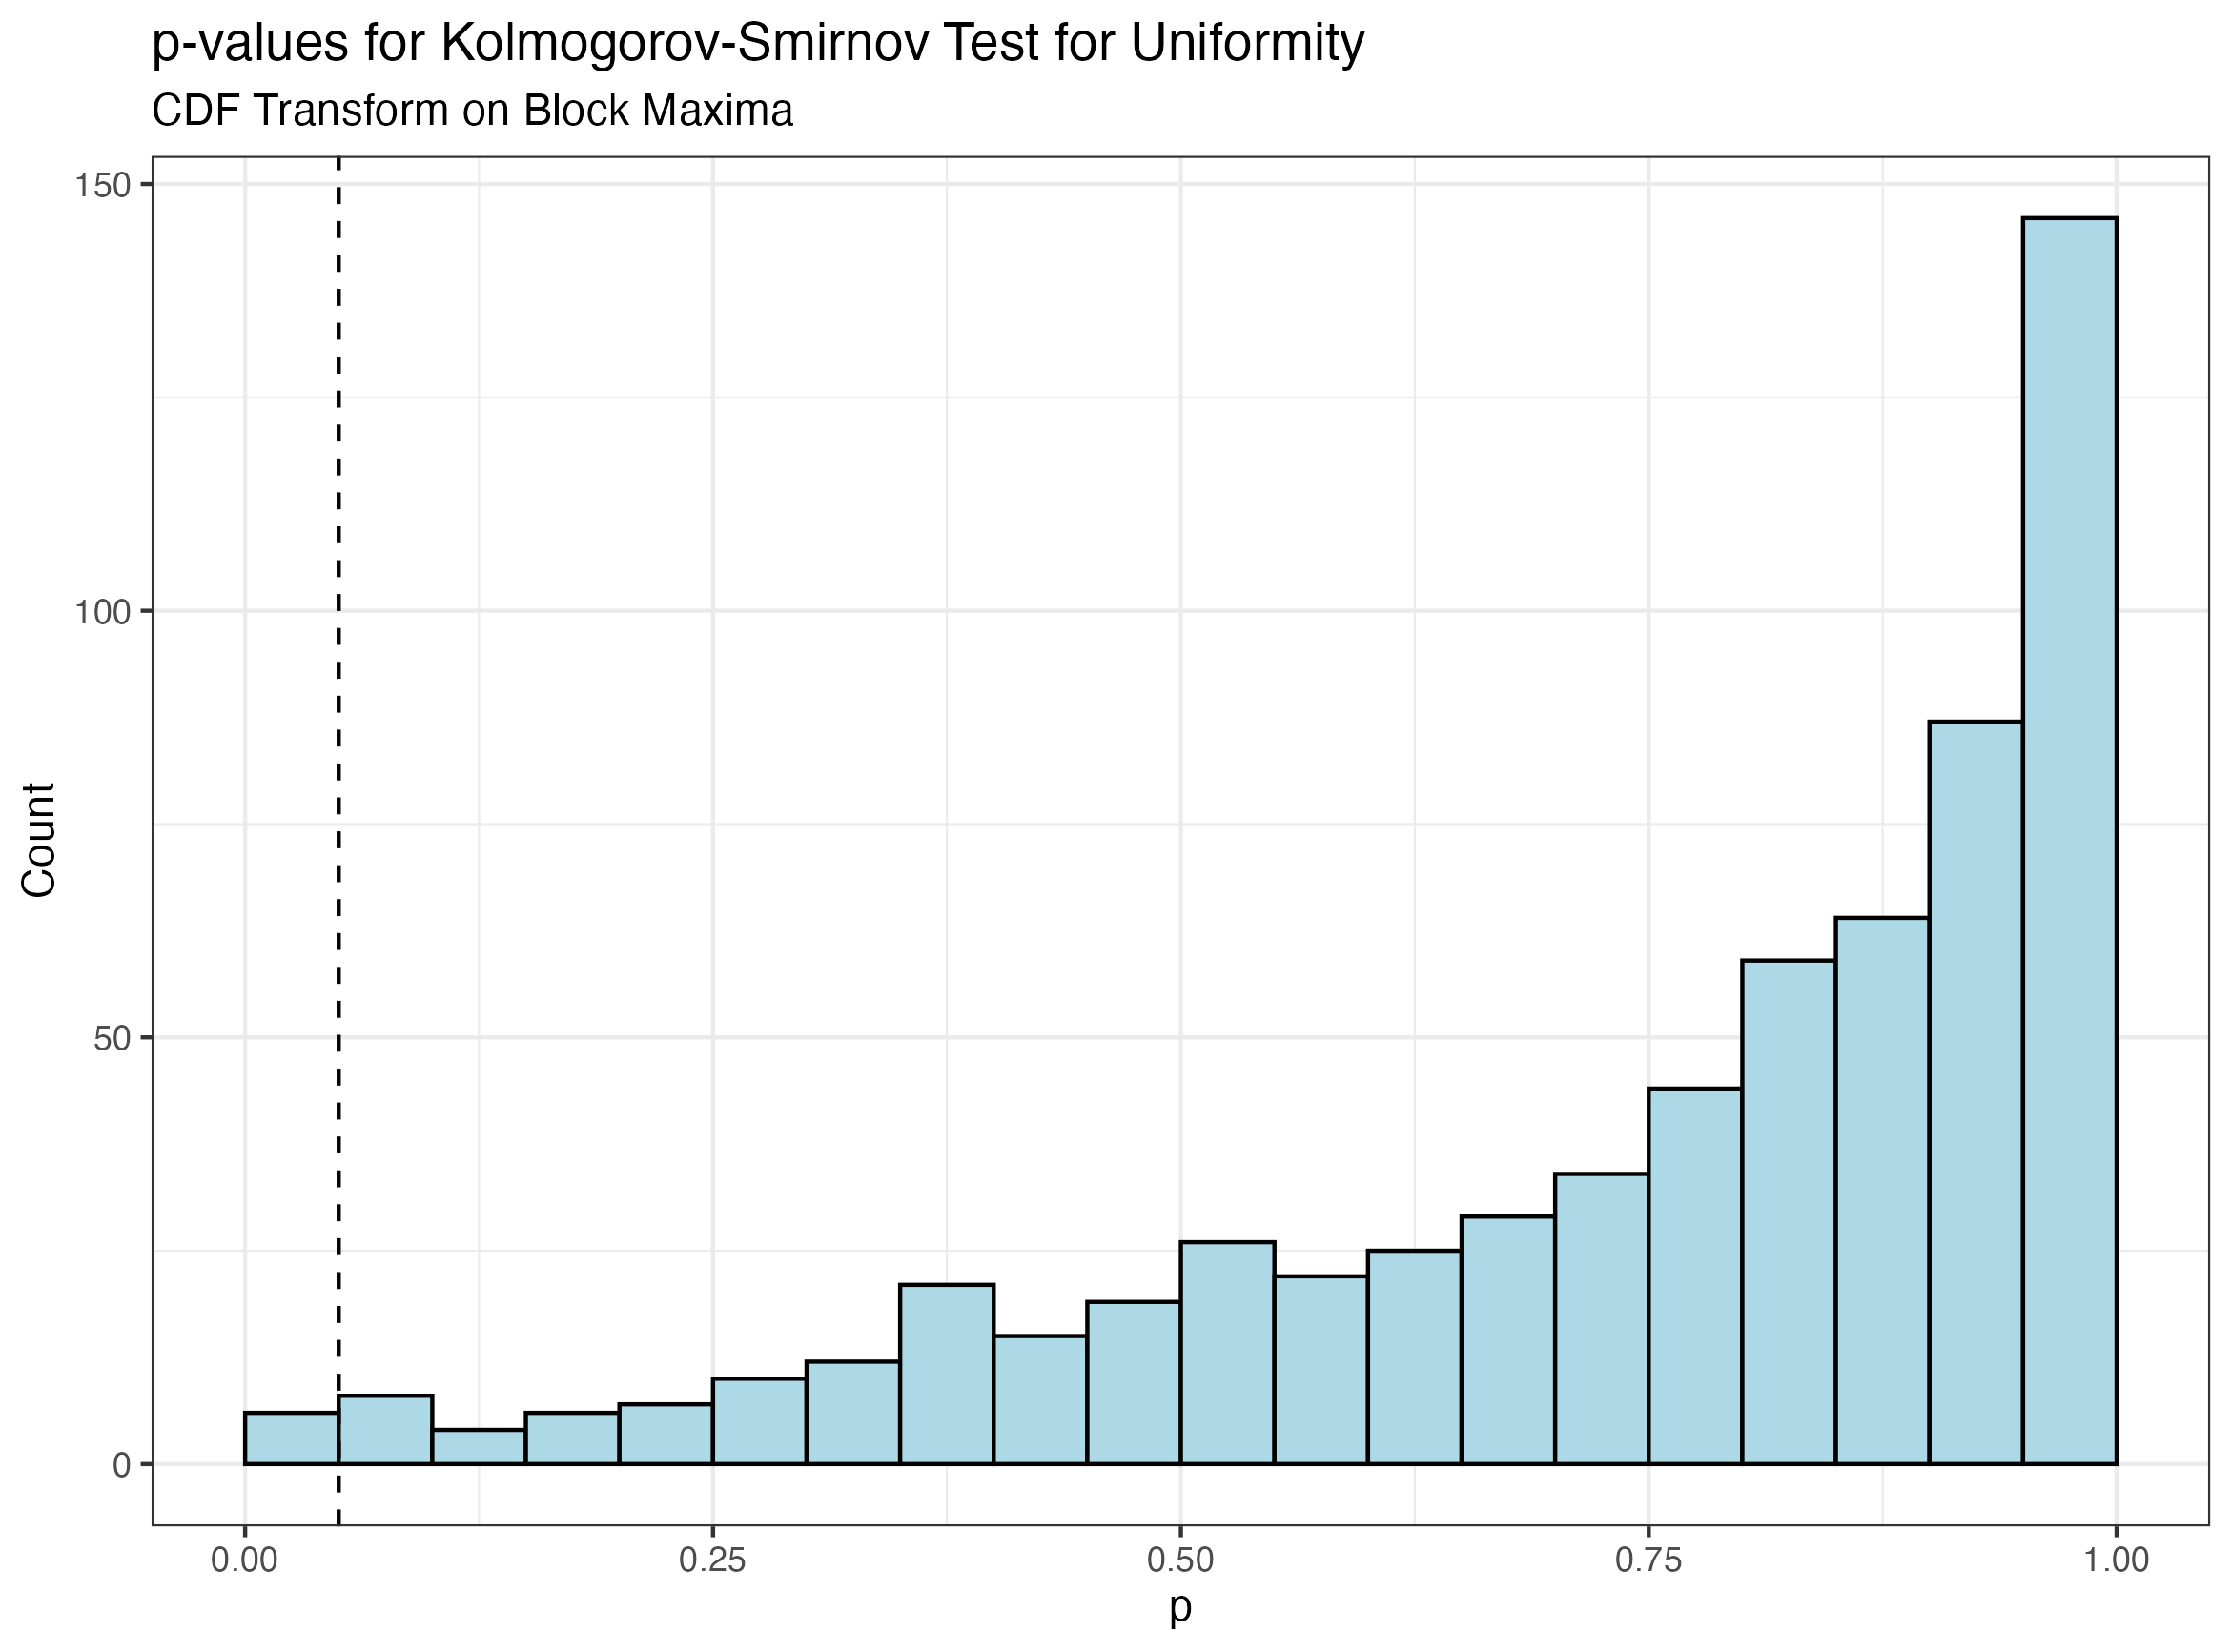
\includegraphics[width=0.75\linewidth]{plots/kstest.png}
    \caption{Evaluating Model Fit}
    \label{fig:ks-test}
\end{figure}

\subsection{Return Levels}
A quantity of interest with the block maxima method is the \textbf{return level}. Usually interpreted in financial contexts, a $k$-block return level represents the quantity one can expect to be exceeded once every $k$ blocks on average. It can be estimated directly using a GEV model, and in this case provides a useful, easy-to-understand statistic to interpret each player EV model. In particular, we can estimate a 5-block return level for each player, representing the EV we can expect them to exceed once every 50 balls in play (BIP), on average.

\chapter{Results and Discussion}\label{ch:results}
\section{Return Level as an EV Metric}
We can now evaluate the quality of 50-BIP return levels as a metric for summarising each player's EV distribution, in particular with respect to the criteria described in section \ref{metrics}.

\begin{figure}[ht]
    \centering
    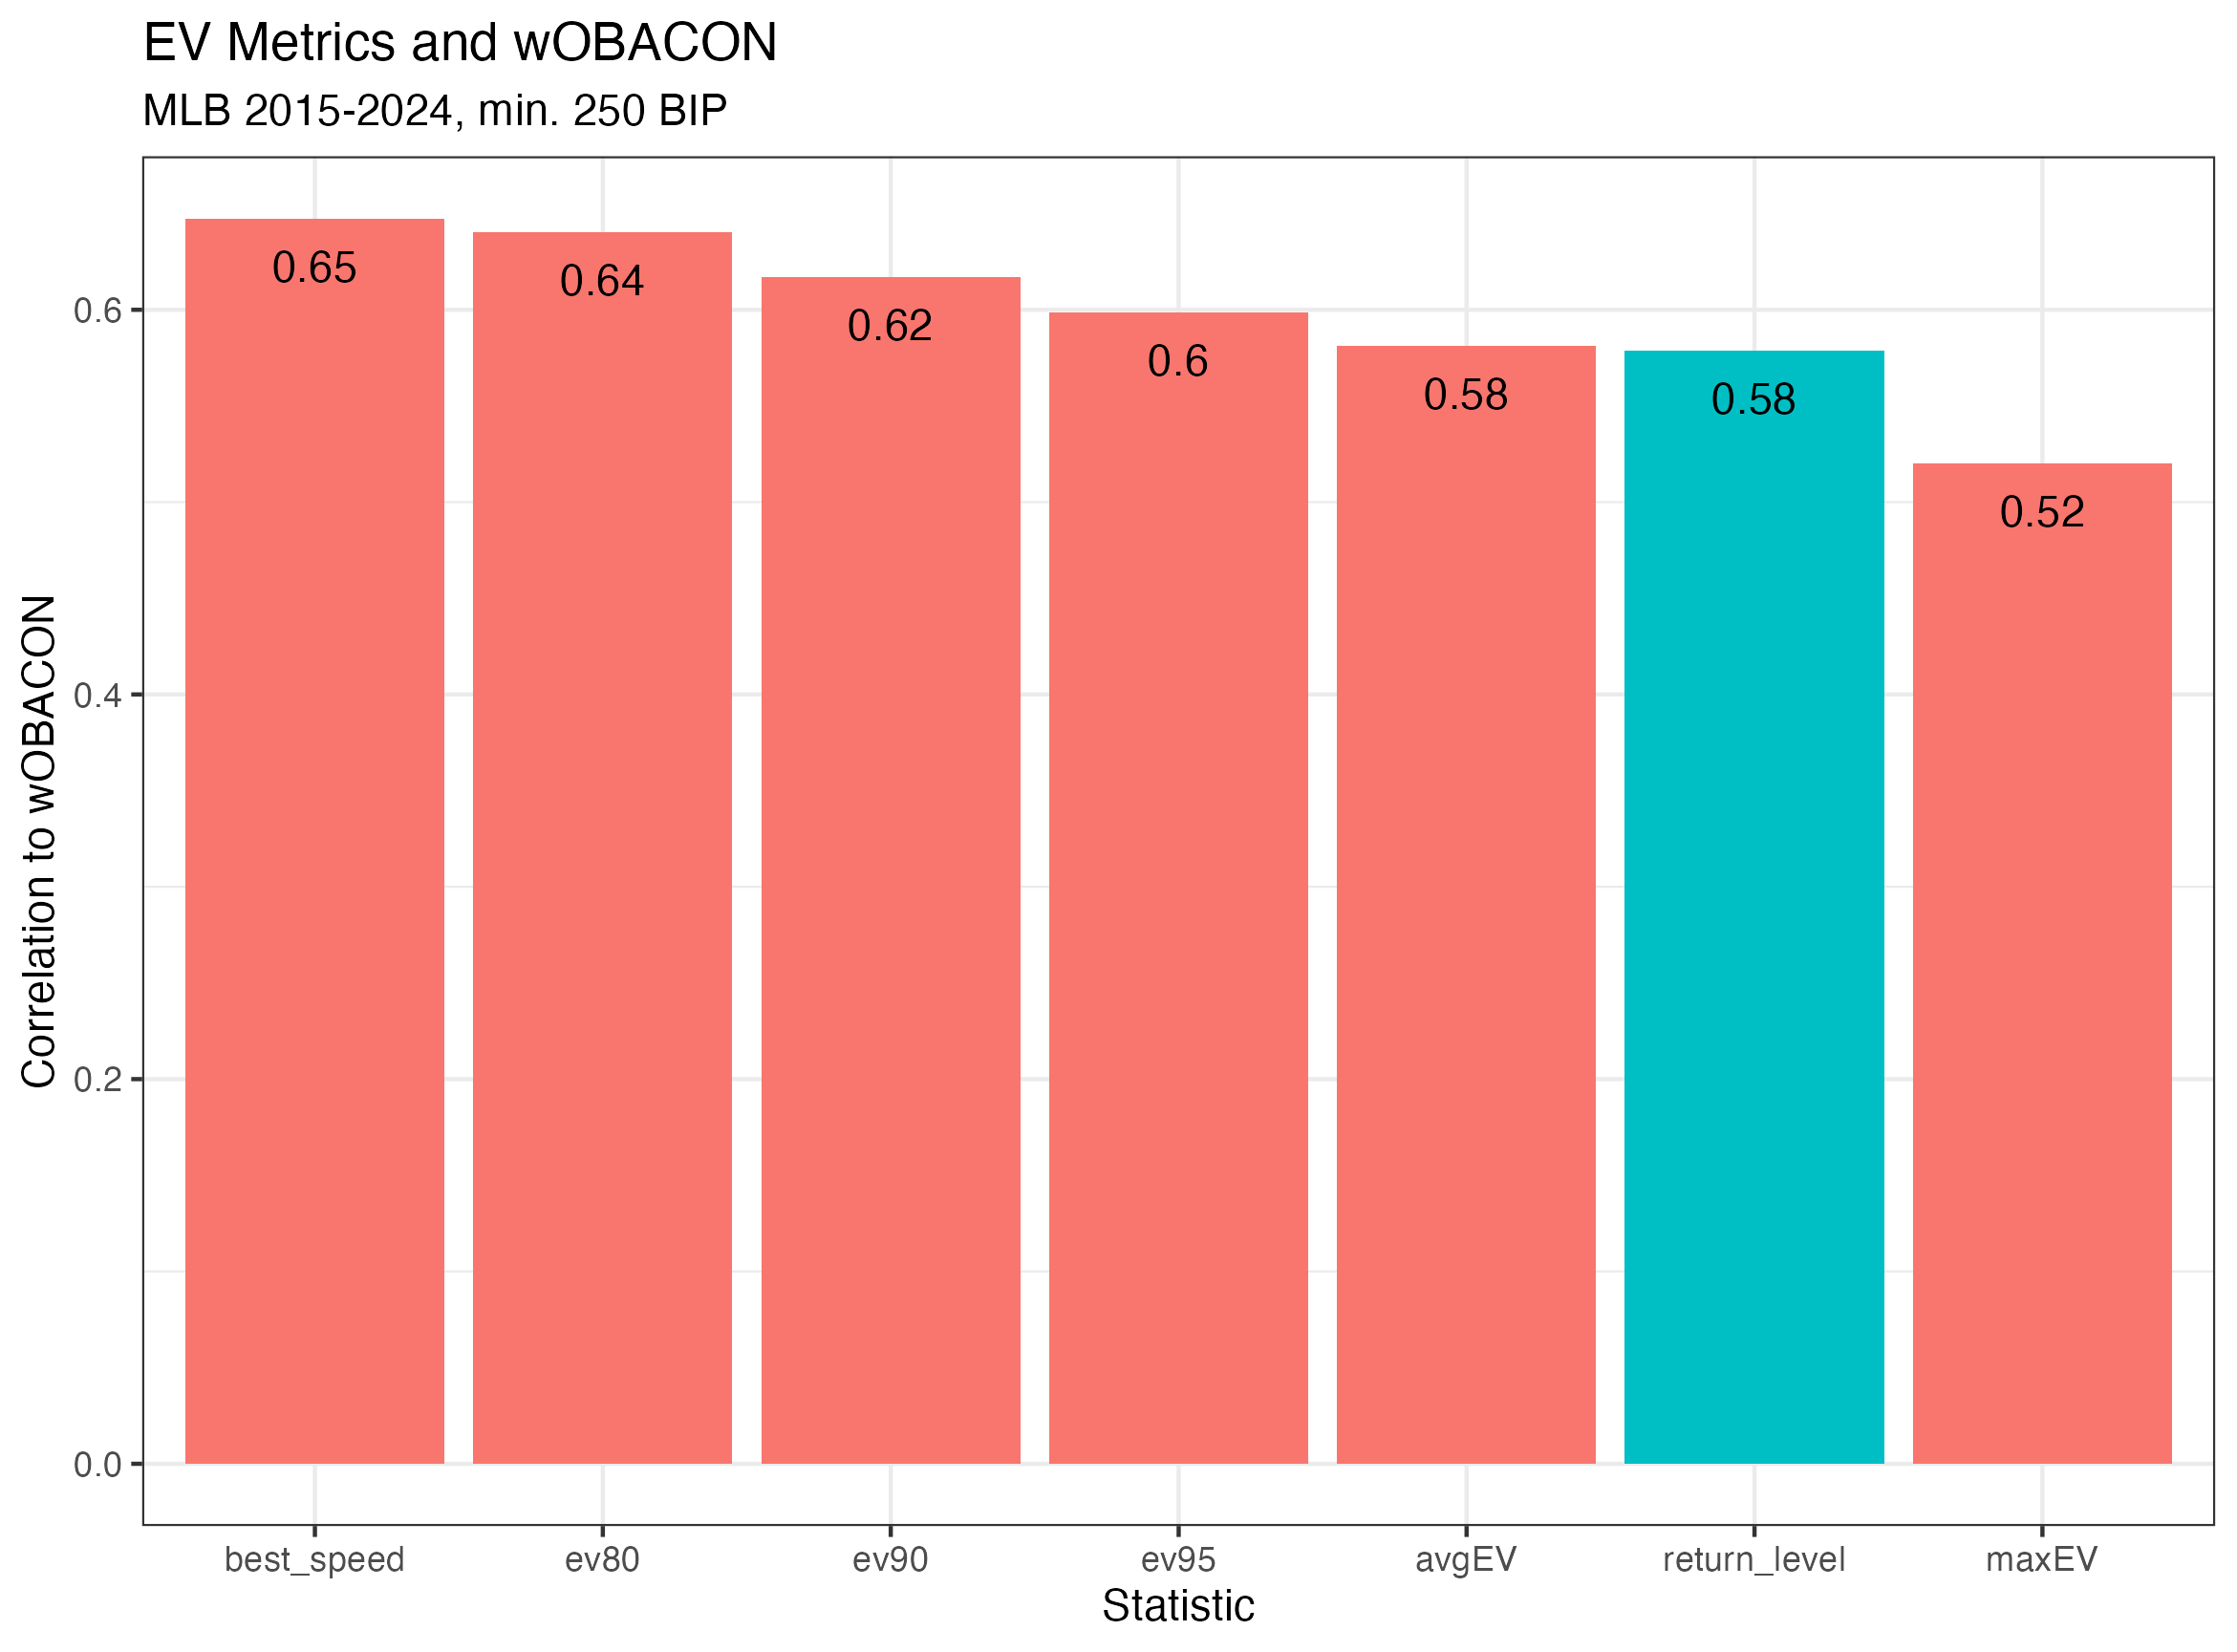
\includegraphics[width=0.85\linewidth]{plots/woba_correlation.png}
    \caption{Correlation with Outcomes}
    \label{fig:corr-outcomes}
\end{figure}

Using wOBACON as the outcome of choice, we first consider how well return levels reflect value of outcomes. 50-BIP return level exhibits a 0.58 correlation coefficient\footnote{Using Pearson's Correlation Coefficient.} with same-season wOBACON. As shown in Figure \ref{fig:corr-outcomes}, this is quite poor performance when compared to other metrics. This is perhaps unsurprising; one big drawback to the block-maxima method is that it ignores a lot of potentially useful information by only using the maximum observation from each block. Given that we are simply evaluating how well return levels describe the data \textit{from which they were estimated}, it is not entirely unusual that they don't perform particularly well.

\begin{figure}[ht]
    \centering
    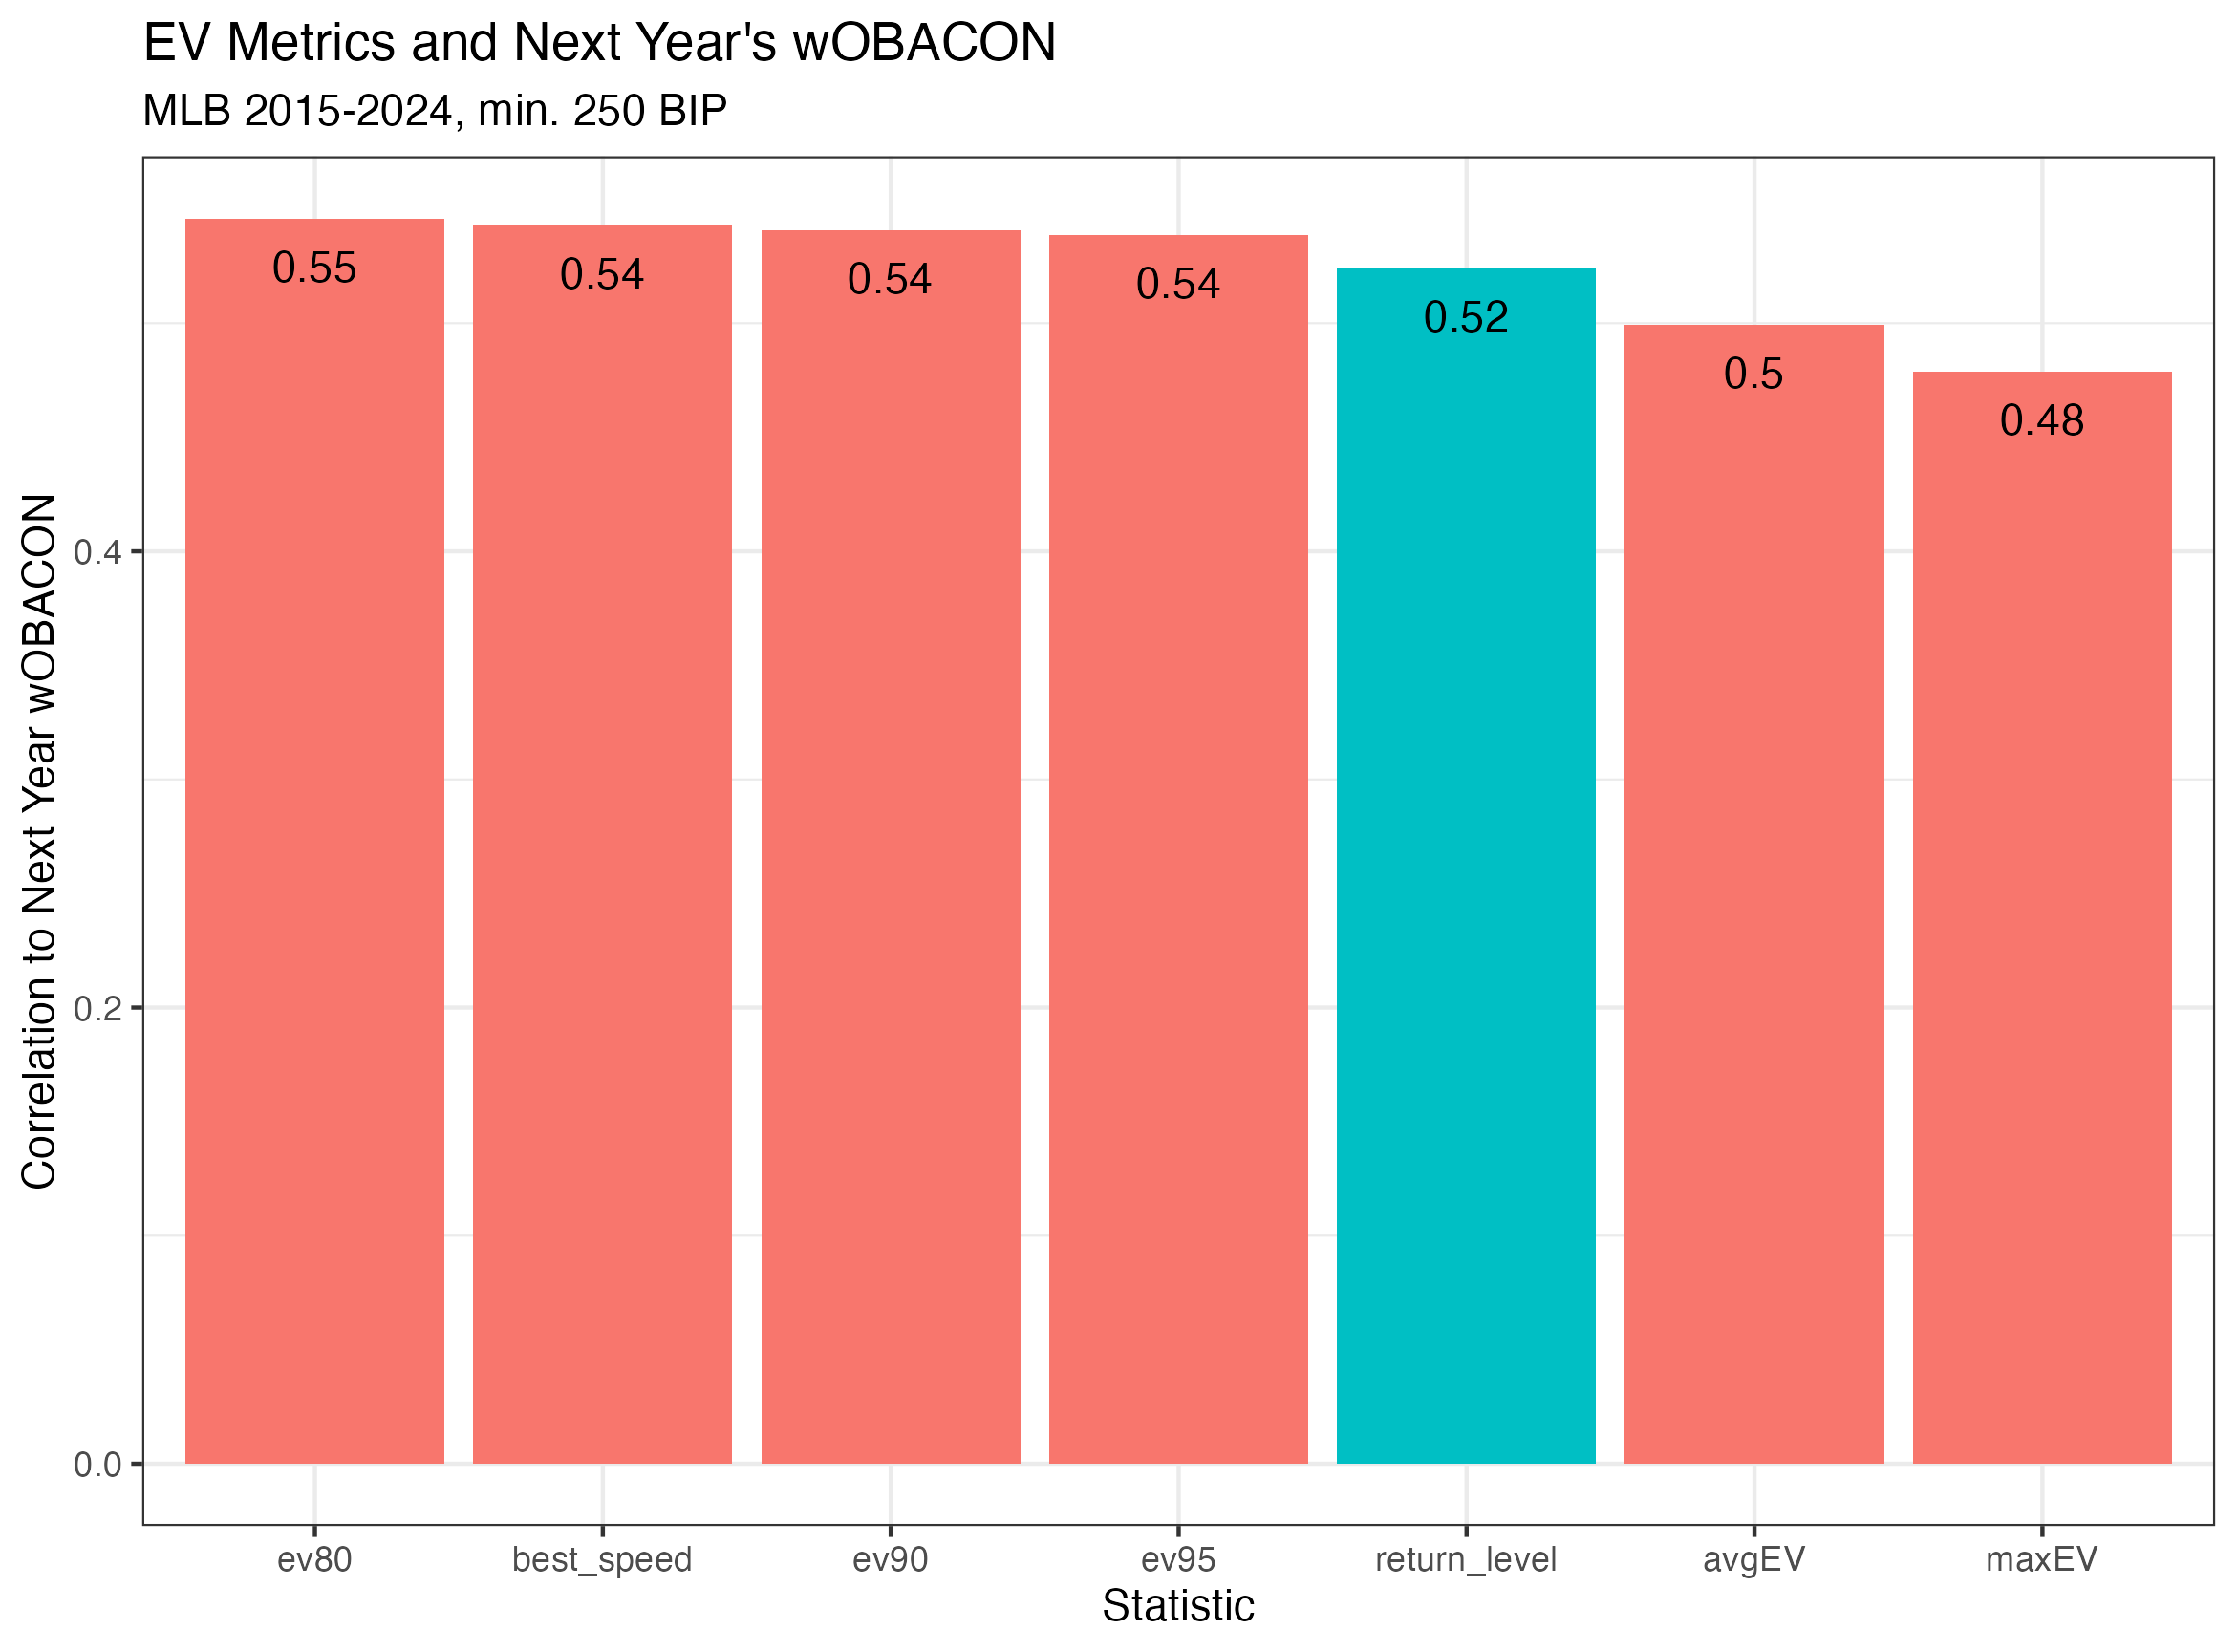
\includegraphics[width=0.85\linewidth]{plots/woba_next_correlation.png}
    \caption{Predictive Power}
    \label{fig:corr-future}
\end{figure}

In terms of predictive value, the 50-BIP return level has a 0.53 correlation with \textit{next} season wOBACON, performing similarly to the best metrics, as shown in Figure \ref{fig:corr-future}. We notice more generally that the EV percentiles and best speed perform significantly better than average EV and maximum EV, with return levels in between.

\begin{figure}[ht]
    \centering
    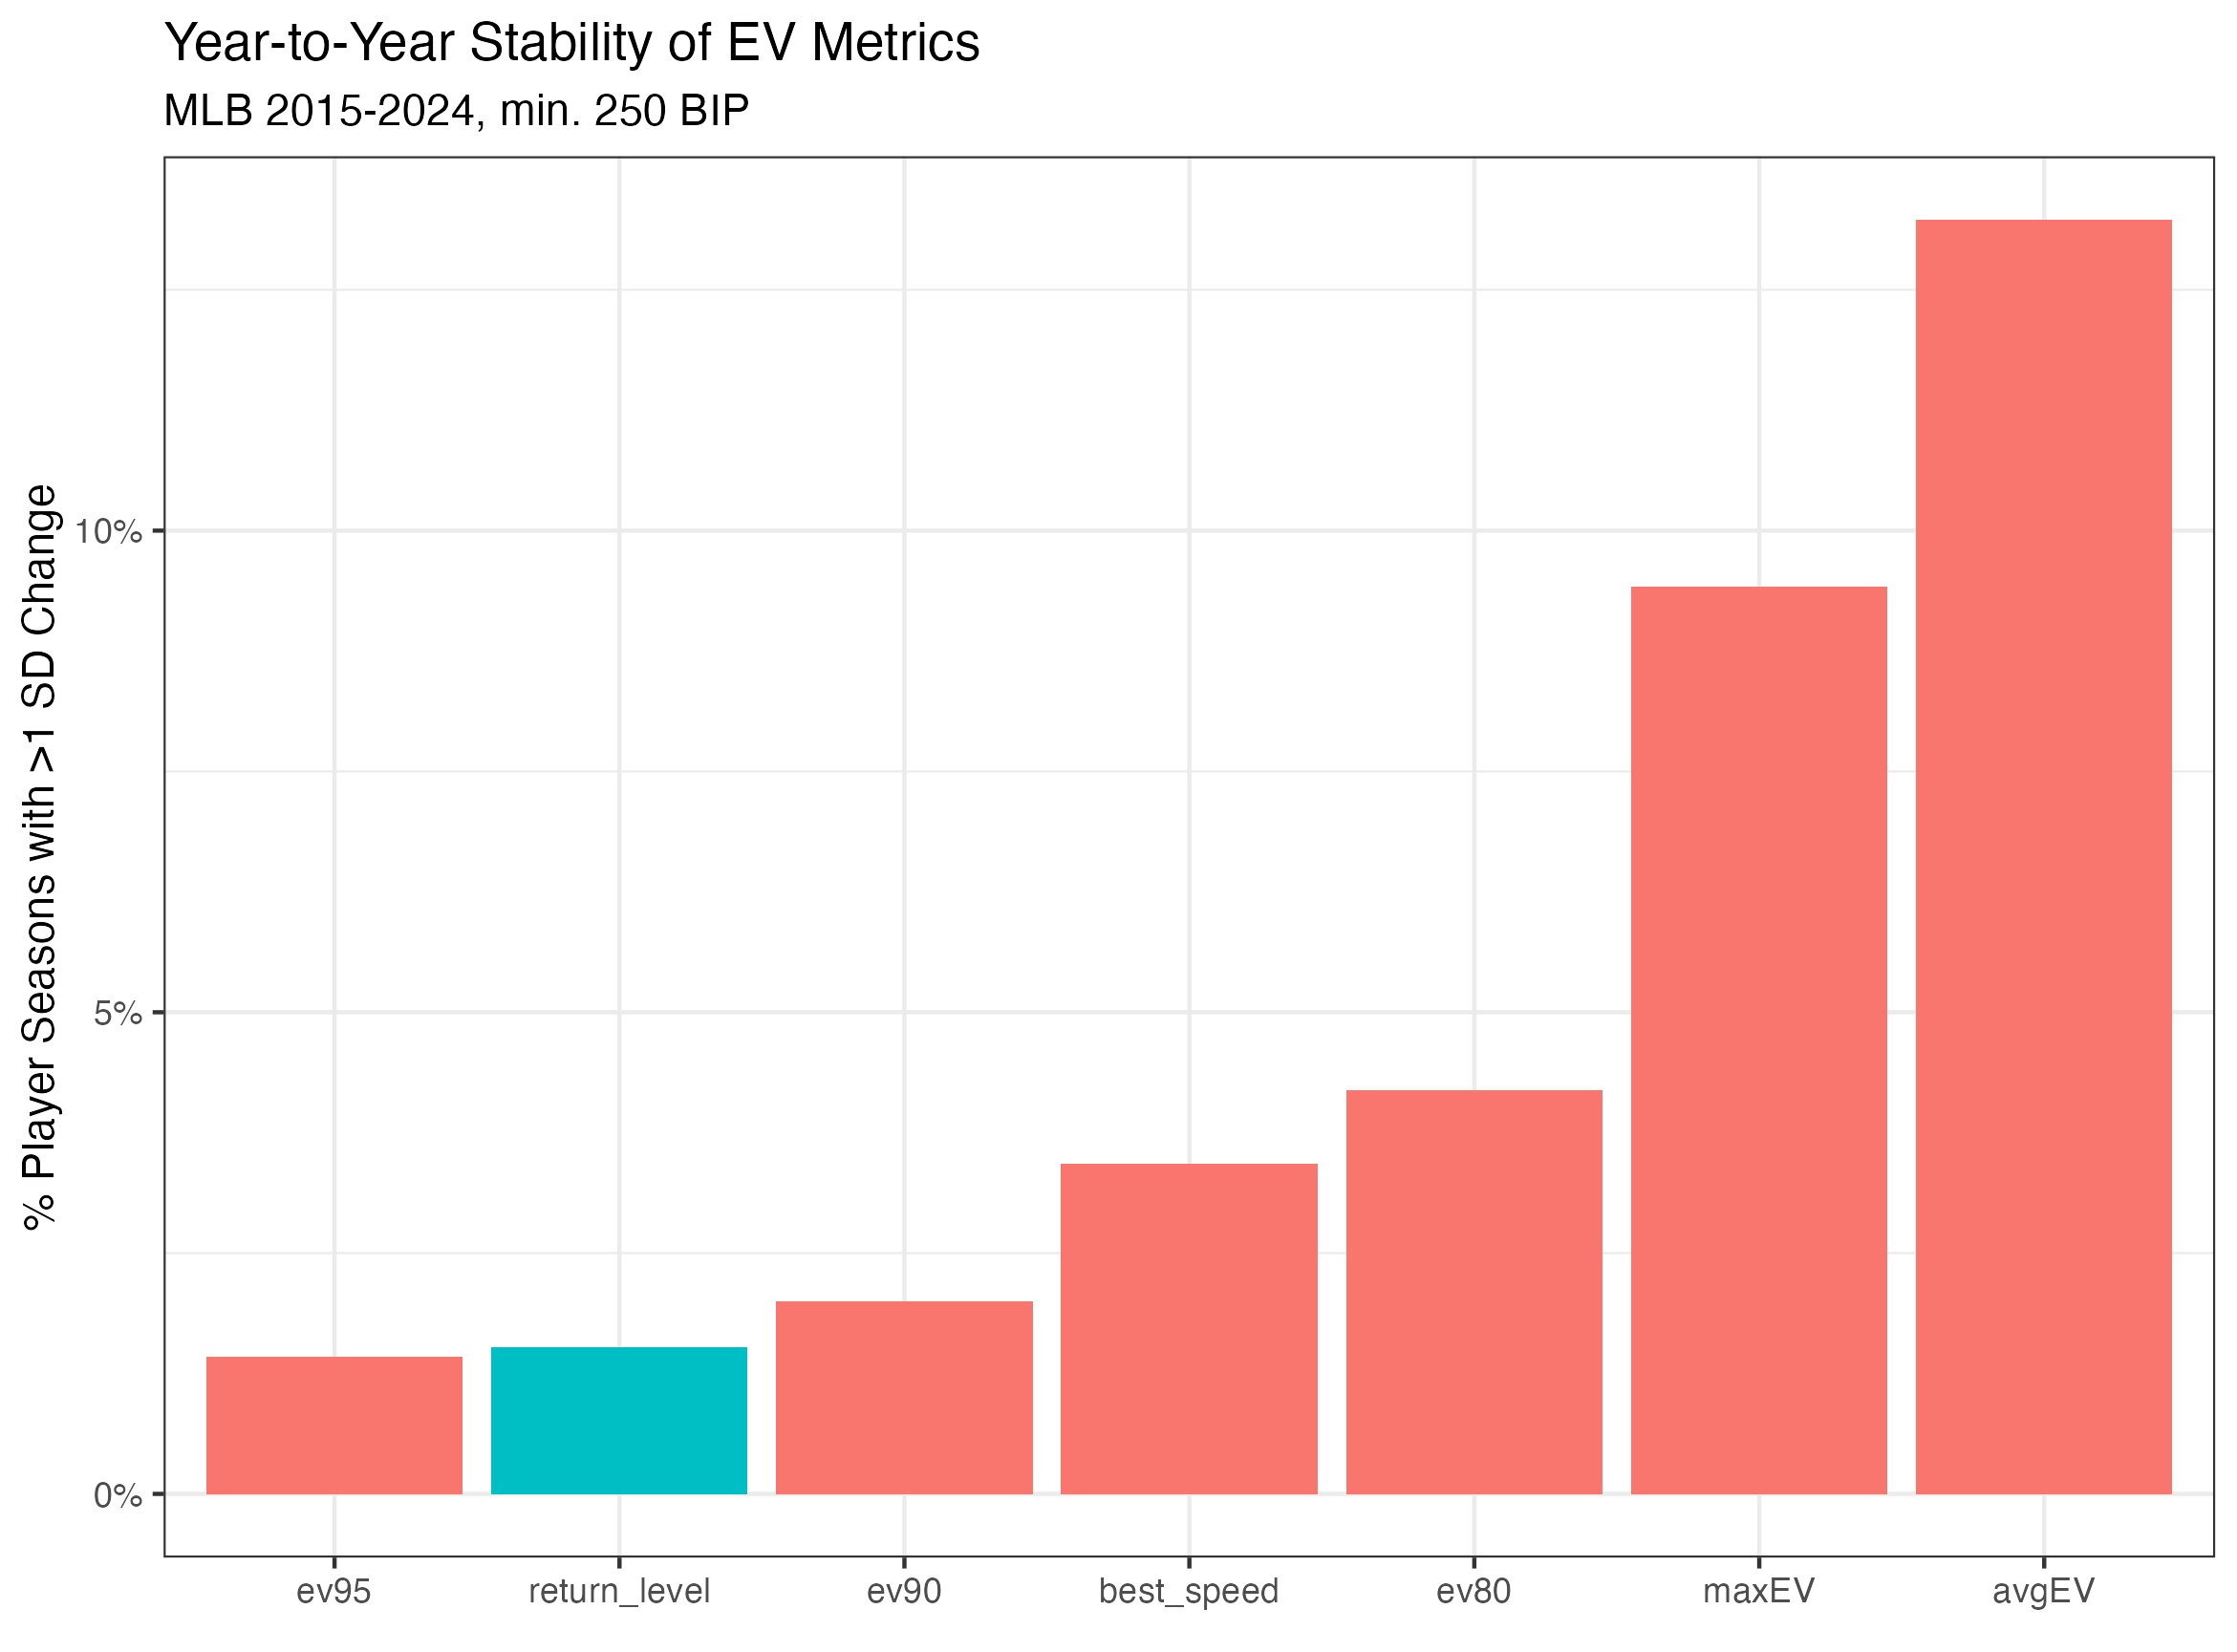
\includegraphics[width=0.7\linewidth]{plots/stability.png}
    \caption{Variance}
    \label{fig:variance}
\end{figure}

Return level separates itself from the other metrics when we consider year-to-year variations. Only 1.5\% of player seasons showed a year-to-year change in return level of more than 1 Standard Deviation. When compared to the variability of the other metrics, return level is second only to EV95 (see Figure \ref{fig:variance}). Whilst best speed is a better descriptor of outcomes and slightly better predictor, it varies more from year to year, rendering it less reliable when evaluating `true' talent. An illustration of the stability of 50-BIP return level is provided in figure \ref{fig:stability}.

\begin{figure}[hb]
    \centering
    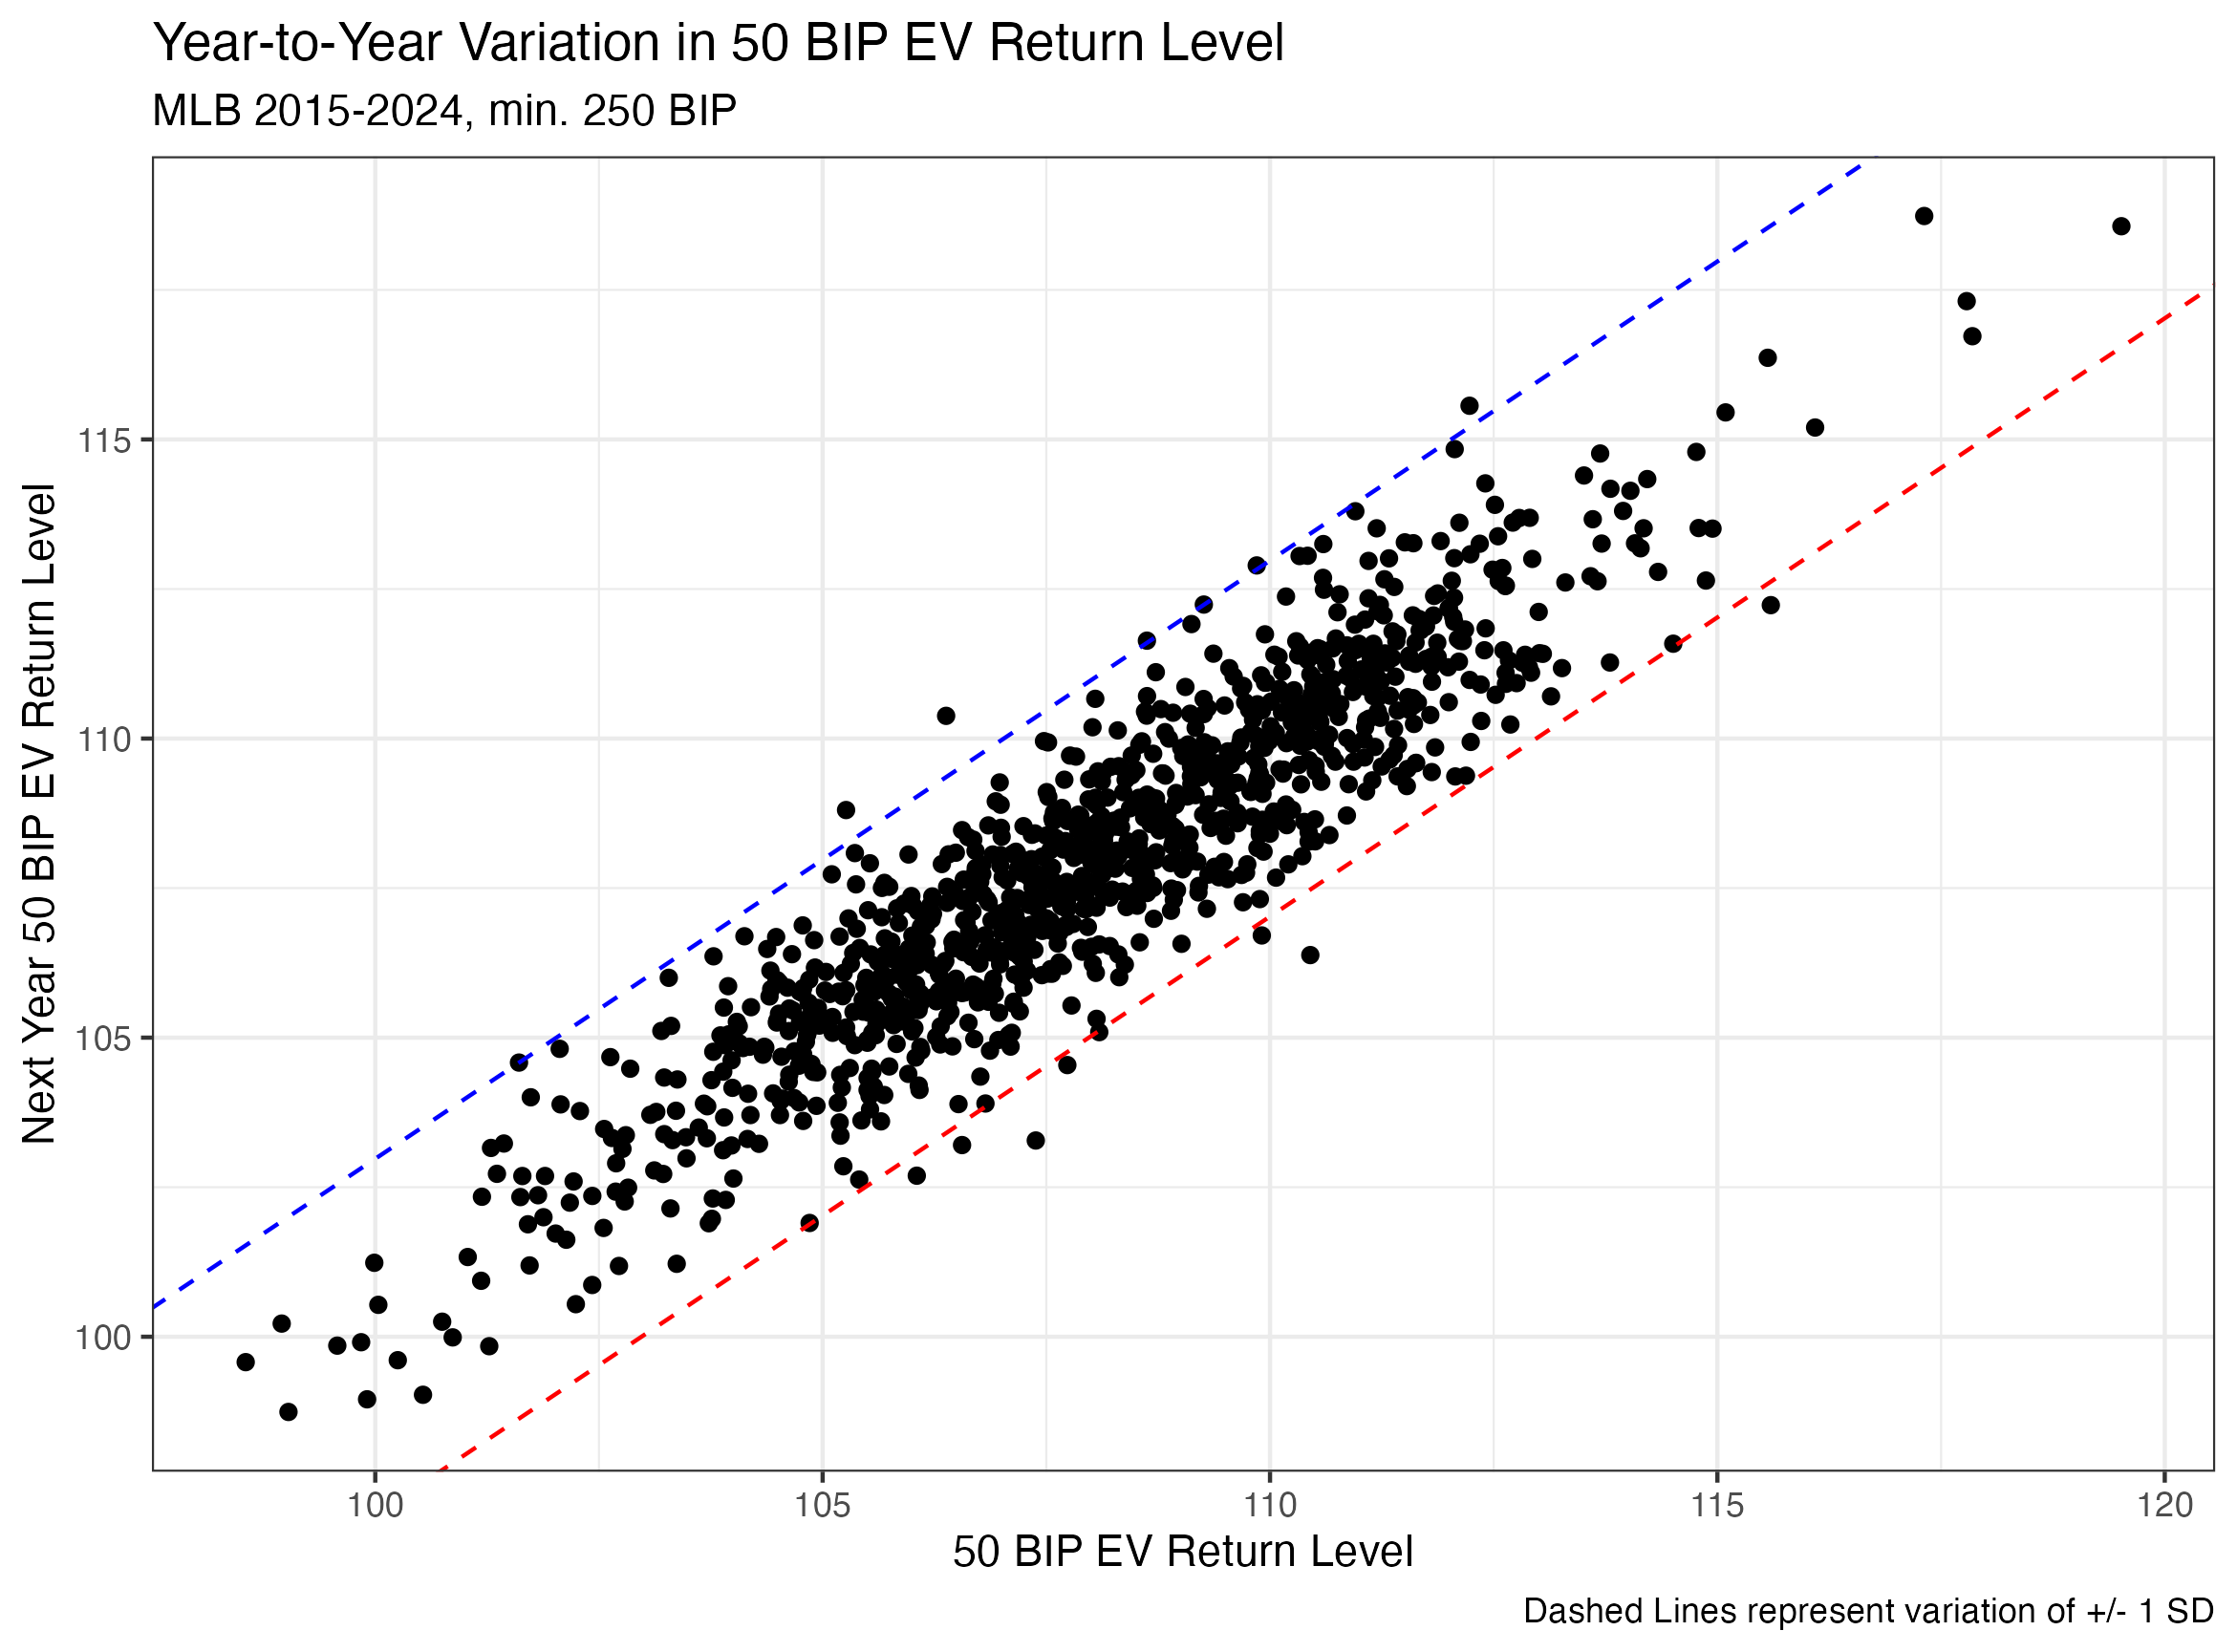
\includegraphics[width=0.7\linewidth]{plots/return_level_stability.png}
    \caption{Stability of 50-BIP Return Level}
    \label{fig:stability}
\end{figure}

\section{Discussion}
50-BIP EV return level performs moderately well as a descriptive metric. It performs similarly to best speed and EV percentiles in predictive power, and is below average for correlation with outcomes. However, its stability is encouraging and sets it apart from the other metrics.

On the other hand, return level has some flaws. It is more computationally intensive than the other metrics, and the sample size required to achieve its demonstrated performance is relatively large. The choice of 10-BIP blocks and 5-block return levels was somewhat arbitrary, and improvements could be made by tuning those `parameters'. Although the metric performs relatively well across the whole sample, some individual models are extremely bad fits due to the estimated $\hat{\xi} < -1$ and non-uniformity of the CDF transform. One solution would be to simply filter out badly-specified models, however a metric which cannot be specified for certain players is definitely problematic. Bayesian inference for GEV models is an active area of research and could aid in the issue of $\hat{\xi} < -1$, by allowing for the imposition of constraints (in this case one could impose $\xi > -1$).

Another area for improvement would be the inclusion of covariates; age in particular. Methods exist for incorporating covariates in GEV models \cite{coles}, however it is unclear how one could implement a general trend over many models. That is, although we fit a separate model for each player-season, an ageing trend is a population-wide effect, not player-specific. Such a problem is beyond the scope of this project, but nevertheless is an interesting area to explore.

\section{Finite Upper Endpoints}
A final point for discussion, unrelated to return levels, is to recall that 
a negative shape parameter bounds the GEV distribution from above. Given that almost all the models estimate a negative shape parameter (see figure \ref{fig:params}), we can infer that each player has a \textit{finite upper endpoint} to their EV distribution. This is an interesting if unsurprising result; we would expect there to be some physical limit to each player's capabilities. Methods for the estimation of the upper endpoint are available \cite{alves2016}, however the estimation is highly dependent on the shape parameter estimate. For $\xi$ close to 0, the endpoint estimate becomes unreasonably high.

Estimating the upper endpoint for each player would be an alternative metric of interest; representing an estimate of their physical limits. However, when estimating the upper endpoint on the fitted player models, the estimates were indeed very unstable with the estimated shape parameter, and as a result don't provide a useful interpretation.

\printbibliography

\end{document}
